%!TEX root = ../apuntesMarkov.tex

\section{Cadenas de Markov a tiempo discreto}

\subsection{Definición, construcción y propiedades básicas}

\subsubsection{Breve recuerdo de probabilidades}

Un \emph{espacio de probabilidad}\MarginNote{Espacio de Probabilidad} es un espacio de medida $(\Omega,\cf,\pp)$ tal que $\pp(\Omega)=1$.
$\pp$ es la \emph{medida de probabilidad}\MarginNote{Medida de Probabilidad}.
Los $A\in\cf$ son los \emph{eventos}.
\lsep
Dado un espacio medible $(S,\cs)$, una \emph{variable aleatoria}\MarginNote{Variable Aleatoria} $X$ a valores en $S$ es una función $X\!:\Omega\longrightarrow S$ que es $\cf$-$\cs$ medible.
\hly{Usualmente nos olvidamos del espacio de probabilidad en la notación}.
Por ejemplo, cuando escribimos $\pp(X\in A)$ a lo que nos referimos es a la medida de la preimagen de $A$ por $X$, es decir
\[\pp(X\in A)=\pp(X^{-1}(A))=\pp(\{\omega\in \Omega\!:X(\omega)\in A\}).\]
Rara vez incluimos los $\omega$'s en la notación, pero es importante mantener la definición formal en mente.
\lsep Dos eventos $A$ y $B$ son \emph{independientes}\MarginNote{Independencia} si $\pp(A\cap B)=\pp(A)\pp(B)$.
La \emph{probabilidad condicional}\MarginNote{Prob. Condicional} de $A$ dado $B$ es
\[\pp(A|B)=\frac{\pp(A\cap B)}{\pp(B)}\]
(asumiendo $\pp(B)>0$; a menudo omitiremos especificar esto cuando hablamos de probabilidades condicionales).
\lsep
Notar que la aplicación $\pp(\cdot|B)\!:\cf\longrightarrow[0,1]$ define una medida de probabilidad\MarginNote{Med. de Prob. sobre un evento B} sobre $(\Omega,\cf,\pp)$ soportada en $B$ (o alternativamente una medida de probabilidad sobre $(B,\cf,\pp)$).
De esta forma, por ejemplo, podemos decir que dados $A,B,C\in\cf$, $A$ y $B$ son \emph{independientes condicionalmente a $C$} si $\pp(A\cap B|C)=\pp(A|C)\pp(B|C)$.
\uexer: Asegúrese de que comprende el contenido de la última frase.

% \begin{mdframed}[style=st_red]
\begin{sqgnote}
Repase la noción de independencia para variables aleatorias y familias de variables aleatorias.
\end{sqgnote}
% \mbox{}\vskip-30pt\mbox{}
\begin{sqgnote}
Repase la definición y propiedades de esperanza condicional, dadas en el Apéndice \ref{sec:espCond}.
\end{sqgnote}
% \end{mdframed}


\subsubsection{Procesos estocásticos y cadenas de Markov}

Dados $(\Omega,\cf,\pp)$ y $(S,\cs)$ como antes, decimos que \hly{una sucesi{\'o}n $(X_n)_{n\geq0}$ de variables aleatorias} es un \emph{proceso estocástico}\MarginNote{Proceso Estocástico}.
Alternativamente uno puede pensar en el proceso estocástico $(X_n)_{n\geq0}$ como una variable aleatoria a valores en el espacio producto $S^\nn$, es decir $X\!:\Omega\longrightarrow S^\nn$ que es $\cf$-$\cs^\nn$ medible, con $\cs^\nn$ dotado de la $\sigma$-álgebra producto.
\lsep
(Más adelante consideraremos procesos estocásticos indexados por $\rr^+$ en vez de $\nn$).
\lsep
El propósito del curso es estudiar un tipo especial pero muy importante de procesos estocásticos: los procesos de Markov.

\vs

En todo lo que sigue $I$\MarginNote{Espacio de Estados} (o a veces $E$) denotará un conjunto numerable, el ``espacio de estados'' donde \hly{nuestros procesos estoc{\'a}sticos tomar{\'a}n valores}.
Sobre $I$ consideramos la $\sigma$-álgebra de las partes $\cp(I)$.
Los elementos de $I$ los denotaremos típicamente por $i,j,k$ o $x,y,z$.
Detrás de todo lo que haremos habrá un espacio de probabilidad fijo $(\Omega,\cf,\pp)$, que solo invocaremos cuando sea necesario.

\begin{defn}\tbf{Cadena de Markov}
Un proceso estocástico $X=(X_n)_{n\geq0}$ a valores en $I$ es un \emph{proceso de Markov a tiempo discreto} o una \emph{cadena de Markov}\MarginNote{Cadena de Markov} si satisface la \emph{propiedad de Markov}:
\begin{equation}\label{eq:propMarkov}
\pp\big(X_{n+1}=i_{n+1}\big|X_0=i_0,\dotsc,X_{n}=i_{n}\big)=\pp\big(X_{n+1}=i_{n+1}\big|X_{n}=i_{n}\big)
\end{equation}\MarginNote{Propiedad de Markov}
para todo $i_0,\dotsc,i_{n+1}\in I$ (que satisfaga $\pp(X_0=i_0,\dotsc,X_{n}=i_{n}\big)>0$).
% Es decir, condicional al presente, el futuro del proceso es independiente del pasado.
\end{defn}

\begin{rem}
La propiedad de Markov es equivalente a decir que $X_{n+1}$ y \NAM[$(X_0,\dotsc,X_{n-1})$]{$(X_0,\dotsc, X_{n-1})$} son independientes condicionales a $X_n$, es decir, ``condicional\MarginNote{Interpretación de la CM} al presente, el futuro del proceso es independiente del pasado''.
\uexer: demuestre esto.
\end{rem}


\begin{prop}\MarginNote{CM a distintos tiempos}
Si $X$ es una cadena de Markov entonces para todo $0\leq t_0\leq\dotsm\leq t_{n+1}$ en $\nn$ y todo $i_0,\dotsc,i_{n+1}\in I$,
\begin{equation}
\pp\big(X_{t_{n+1}}=i_{n+1}\big|X_{t_0}=i_0,\dotsc,X_{t_n}=i_{n}\big)=\pp\big(X_{t_{n+1}}=i_{n+1}\big|X_{t_n}=i_{n}\big).
\end{equation}
\end{prop}
\vskip
\begin{proof}
\uexer.
\end{proof}

\begin{ex}\tbf{Marcha aleatoria simple en $\zz$}\label{ex:marchaZ}\MarginNote{Marcha Aleatoria Simple en $\zz$}
Una partícula o individuo camina por $\zz$ de la siguiente forma.
A tiempo $0$ comienza en $X_0=x\in\zz$.
Luego en cada instante de tiempo decide dar un paso a la derecha con probabilidad $p\in[0,1]$ y un paso a la izquierda con probabilidad $1-p$, todo de manera independiente, es decir, para cada $n\geq1$ tenemos
\[X_n=\begin{dcases*}
X_{n-1}+1 & con probabilidad $p$,\\
X_{n-1}-1 & con probabilidad $1-p$.
\end{dcases*}\]
Entonces $(X_n)_{n\geq0}$ es una cadena de Markov (\uexers: chequee esto).
\lsep
Por ahora esta descripción es informal, luego veremos como se puede construir esta cadena de manera rigurosa.
\end{ex}

\begin{ex}\tbf{Ruina del jugador}\label{ex:ruina}\MarginNote{Ruina del jugador}
Consideramos ahora un juego de apuestas, donde en cada turno el jugador gana $1$ con probabilidad $p$ y pierde $1$ con probabilidad $1-p$.
El jugador para de jugar si se queda sin dinero.
Esto es muy similar a la cadena anterior, excepto que ahora el espacio de estados es $\zz_{\geq0}$ y tenemos
\[X_n=\begin{dcases*}
X_{n-1}+1 & con probabilidad $p$ si $n>0$,\\
X_{n-1}-1 & con probabilidad $1-p$ si $n>0$,\\
0 & con probabilidad $1$ si $n=0$.
\end{dcases*}\]
\end{ex}

\begin{ex}\tbf{Cadena de Ehrenfest}\label{ex:ehrenfest}\MarginNote{Cadena de Ehrenfest}
En este ejemplo nos imaginamos una caja rectangular dividida en dos cámaras que están conectadas por un pequeño orificio, donde $r$ moléculas de aire se mueven libremente al azar.
\begin{figure}[h]
\centering
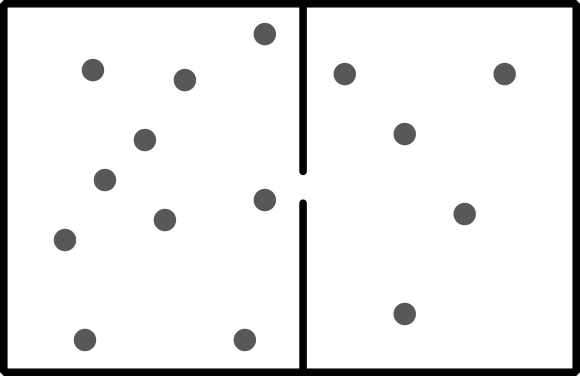
\includegraphics[width=1.6in]{figures/ehrenfest.png}
\end{figure}
P. Ehrenfest propuso a comienzos del sigo XX el siguente modelo para estudiar esta situación.
Tenemos $r$ bolas distribuidas en 2 dos urnas, una con $k$ bolas (la cámara izquierda de la caja) y la otra con las restantes $r-k$ (la cámara derecha).
Luego en cada instante de tiempo tomamos una de las $r$ bolas elegida uniformemente al azar y la cambiamos de urna.
La cadena de Markov detrás de este ejemplo es la siguiente: $I=\{0,\dots,r\}$ y, para $n\geq1$, tenemos
\[X_n=\begin{dcases*}
X_{n-1}+1 & con probabilidad $\frac{r-X_{n-1}}{r}$,\\
X_{n-1}-1 & con probabilidad $\frac{X_{n-1}}{r}$.
\end{dcases*}\]
\end{ex}


\begin{defn}\tbf{Cadena de Markov homogénea, matriz de transición}\MarginNote{CM Homogénea}
Sea $X$ una cadena de Markov.
Decimos que $X$ es \emph{homogénea} si
\[\pp(X_{m+1}=j|X_m=i)=\pp(X_{n+1}=j|X_n=i)\quad\forall~m,n\geq0,~i,j\in I.\]
En este caso a la matriz $P=\big(p_{ij}\big)_{i,j\in I}$\MarginNote{Matriz de Transición} dada por $p_{ij}=\pp(X_{1}=j|X_0=i)$ le llamamos \emph{matriz de transición} de la cadena de Markov $X$; $p_{ij}$\MarginNote{Prob. de Transición} es la \emph{probabilidad de transición de $i$ a $j$}.
\end{defn}

\begin{ex}
La marcha aleatoria simple del Ejem. \ref{ex:marchaZ} es una cadena de Markov homogénea, y su matriz de transición $P$ está dada por
\[p_{ij}=\begin{dcases*}
p & si $j=i+1$,\\
1-p & si $j=i-1$,\\
0 & cualquier otro $j$.
\end{dcases*}\]
\end{ex}

\begin{exer}
Escriba la matriz de transición asociada a la cadena de Ehrenfest introducida en el Ejemplo \ref{ex:ehrenfest}.
\end{exer}

Notar que $P$ es una matriz \hly{indexada por un conjunto numerable}, pero esto no nos traerá mayores dificultades (lo discutiremos en más detalle más adelante).
$P$ no puede ser cualquier matriz, si no que claramente debe satisfacer algunas propiedades especiales, precisamente:

\begin{defn}\tbf{Matriz estocástica}
Una matriz $P=\big(p_{ij}\big)_{i,j\in I}$ se dice \MarginNote{Matriz Estocástica}\emph{matriz estocástica} si:\\[-20pt]
\begin{itemize}
\item $p_{ij}\geq0$ para todo $i,j\in I$.
\item $\sum_{j\in I}p_{ij}=1$ para todo $i\in I$.
\end{itemize}
En otras palabras, $P$ es una matriz estocástica si para cada $i\in I$, $(p_{ij})_{j\in I}$ es un vector de probabilidad.
\end{defn}

\begin{prop}\MarginNote{Matr. de Trans. de CM es Matr. Est.}
Si \hlg{$P$ es la matriz de transici{\'o}n de una cadena de Markov}, entonces \hlo{$P$ es matriz estoc{\'a}stica}.
\end{prop}

\vskip

\begin{proof} 
\uexer~(fácil).
\end{proof} 

Durante el curso estaremos interesados casi exclusivamente \hlo{en el caso de cadenas de Markov homog{\'e}neas}.
Por lo tanto, en todo lo que sigue trabajaremos bajo la siguiente convención:
\begin{quote}
% \begin{mdframed}[style=st_red]
\MarginNote{Todas las CM son homogéneas (convención)}Salvo en los casos puntuales en que se indique lo contrario, todas las cadenas de Markov que aparezcan en estas notas serán consideradas implícitamente como cadenas homogéneas.
% \end{mdframed}
\end{quote}

\vskip1pt

\begin{exer}
Sea $X$ una cadena de Markov no homogénea a valores en $I$.
Encuentre una cadena de Markov $\tilde X$ a valores en $I\times\nn$ que es homogénea y que permite recuperar la distribución de la cadena original $X$. 
\end{exer}

\subsubsection{Caracterización y construcción}

\hly{La matriz de transici{\'o}n gobierna la evoluci{\'o}n de nuestra cadena de Markov $X$}.
Para determinar la distribución de la cadena hace falta un ingrediente más:

\begin{defn}\tbf{Distribución inicial}\MarginNote{Distribución Inicial}
Al vector de probabilidad $\mu$ sobre $I$ definido por $\mu_i=\pp(X_0=i)$ le llamamos la \emph{\hlo{distribuci{\'o}n inicial}} de la cadena de Markov~$X$.
\end{defn}

\hly{Usaremos indistintamente la notaci{\'o}n $\mu$ para un vector de probabilidad} como en la definición y para una medida de probabilidad sobre $I$, que en cualquier caso son la misma cosa.

Es relativamente fácil ver que toda cadena de Markov, y en particular sus distribuciones finito-dimensionales, \hly{queda determinada por su matriz de transici{\'o}n y su distribuci{\'o}n inicial}:

\begin{prop}\label{prop:caractMarkov}\MarginNote{Caracterización de una Cadena de Markov}
$X$ es una cadena de Markov con matriz de transición $P$ y distribución inicial $\mu$ si y solo si
\[\pp(X_0=i_0,X_1=i_1,\dotsc,X_n=i_n)=\mu_{i_0}p_{i_0i_1}\dotsc p_{i_{n-1}i_n}.\]
\end{prop}

\begin{proof}
Para la primera implicancia escribimos
\NAM[
\begin{align}
\pp(X_0=i_0,\dotsc,X_n=i_n)
&=\pp(X_n=i_n|X_{n-1}=i_{n-1},\dotsc,X_0=i_0)\pp(X_{n-1}=i_{n-1},\dotsc,X_0=i_0)\hspace{-16pt}\\
&=\pp(X_n=i_n|X_{n-1}=i_{n-1})\pp(X_{n-1}=i_{n-1},\dotsc,X_0=i_0)\\
&=p_{i_{n-1}i_n}\pp(X_{n-1}=i_{n-1},\dotsc,X_0=i_0),\\
\shortintertext{donde en la segunda igualdad usamos la propiedad de Markov, y luego repetimos inductivamente hasta}
&=p_{i_{n-1}i_n}p_{i_{n-2}i_{n-1}}\dotsm p_{i_1i_0}\pp(X_0=i_0)\\
&=p_{i_{n-1}i_n}p_{i_{n-2}i_{n-1}}\dotsm p_{i_1i_0}\mu_{i_0},
\end{align}
]{
\begin{align}
\pp(X_0=i_0,\dotsc,X_n=i_n)
&=\pp(X_n=i_n|X_{n-1}=i_{n-1},\dotsc,X_0=i_0) \\
&\qquad \qquad \qquad \qquad \qquad \qquad \cdot \pp(X_{n-1}=i_{n-1},\dotsc,X_0=i_0)\hspace{-16pt}\\
&=\pp(X_n=i_n|X_{n-1}=i_{n-1})\pp(X_{n-1}=i_{n-1},\dotsc,X_0=i_0)\\
&=p_{i_{n-1}i_n}\pp(X_{n-1}=i_{n-1},\dotsc,X_0=i_0),\\
\shortintertext{donde en la segunda igualdad usamos la propiedad de Markov, y luego repetimos inductivamente hasta}
&=p_{i_{n-1}i_n}p_{i_{n-2}i_{n-1}}\dotsm p_{i_1i_0}\pp(X_0=i_0)\\
&=p_{i_{n-1}i_n}p_{i_{n-2}i_{n-1}}\dotsm p_{i_1i_0}\mu_{i_0},
\end{align}
}
que es lo que buscábamos.

Para la conversa, probemos primero que $X$ es cadena de Markov, es decir, que satisface la propiedad de Markov.
Usando la hipótesis tenemos
\begin{align}
\pp(X_{n+1}=i_{n+1}|X_{i_n},\dotsc,X_0=i_0)&=\frac{\pp(X_{n+1}=i_{n+1},\dotsc,X_0=i_0)}{\pp(X_{i_n},\dotsc,X_0=i_0)}\\
&=\frac{\mu_{i_0}p_{i_0i_1}\dotsc p_{i_{n}i_{n+1}}}{\mu_{i_0}p_{i_0i_1}\dotsc p_{i_{n-1}i_n}}=p_{i_{n}i_{n+1}}.
\end{align}
Por otro lado tenemos
\begin{align}
\pp(X_{n+1}=i_{n+1}|X_n=i_n)&=\frac{\pp(X_{n+1}=i_{n+1},X_n=i_n)}{\pp(X_n=i_n)}\\
&\textstyle=\frac1{\pp(X_n=i_n)}\sum_{i_0,\dotsc,i_{n-1}\in I}\pp(X_{n+1}=i_{n+1},\dotsc,X_0=i_0)\\
&\textstyle=\frac1{\pp(X_n=i_n)}\sum_{i_0,\dotsc,i_{n-1}\in I}\mu_{i_0}p_{i_0i_1}\dotsm p_{i_{n-1}i_{n}}p_{i_{n}i_{n+1}}\\&
\textstyle=\frac1{\pp(X_n=i_n)}\sum_{i_0,\dotsc,i_{n-1}\in I}\pp(X_0=i_0,\dotsc,X_{n}=i_{n})p_{i_{n}i_{n+1}},
\end{align}
donde usamos probabilidades totales y luego la hipótesis nuevamente.
Dejando el factor $p_{i_{n}i_{n+1}}$ afuera, la última suma vale $\pp(X_n=i_n)$, y entonces deducimos que $\pp(X_{n+1}=i_{n+1}|X_n=i_n)=p_{i_{n}i_{n+1}}$.
Juntando con lo anterior, esto nos da la propiedad de Markov, y además nos dice que $P$ es la matriz de transición de la cadena.
Falta derivar la condición inicial, pero esto es directo de la hipótesis, tomando $n=1$ y sumando sobre $i_1\in I$ (\uexers: hágalo).
\end{proof}

Es natural preguntarse ahora por la conversa al resultado anterior: dados un vector de probabilidad $\mu$ y una matriz estocástica $P$, ¿existe una cadena de Markov con condición inicial $\mu$ y matriz de transición $P$? El siguiente teorema nos da una respuesta afirmativa a esta pregunta

\begin{thm}\tbf{Existencia de una cadena de Markov con $\mu$ y $P$ dados}\MarginNote{Exist. de una CM con $\mu$ y $P$ dados}
Sea $\mu$ una medida de probabilidad sobre $I$ y $P$ una matriz estocástica indexada por $I$.
Entonces existe un espacio de probabilidad $(\Omega,\cf,\pp)$ y una sucesión $X=\big(X_n\big)_{n\geq0}$ de variables aleatorias en este espacio tal que $X$ es una cadena de Markov con distribución inicial $\mu$ y matriz de transición $P$.
\end{thm}

\hly{La construcci{\'o}n de una cadena de Markov como en el teorema no es {\'u}nica}.
En la demostración usaremos la que se conoce como la \emph{construcción canónica}, después veremos otra que también es importante.

\begin{sqgnote}
Repase el Teorema de Consistencia de Kolmogorov (ver, por ej., \cite{medidaJSM}).
\end{sqgnote}

\begin{proof}
Partimos eligiendo $\Omega$ como $I^\nn$ y $\cf=\cp(I)^\nn$ (la $\sigma$-álgebra producto); $(\Omega,\cf)$ elegidos así es el ``espacio medible canónico'' para la construcción de una cadena de Markov con $\mu$ y $P$ dados.
Para definir $\pp$ especificamos su valor sobre cilindros mediante
\begin{equation}\label{eq:cyl1}
\pp\big(\{\omega\in I^\nn\!:\omega_{0}=i_0,\dotsc,\omega_n=i_n\}\big)=\mu_{i_0}p_{i_0i_1}\dotsm p_{i_{n-1}i_n}.
\end{equation}
Usando el Teorema de Consistencia de Kolmogorov se tiene que existe una única medida de probabilidad $\pp$ sobre todo $I^\nn$ que satisface \eqref{eq:cyl1}.

\begin{exer}
Verificar esto.
\end{exer}

\noindent Ahora definimos la variable aleatoria $X_n\!:\Omega\longrightarrow I$ mediante
\[X_n(\omega)=\omega_n.\]
Por construcción se tiene entonces que
\begin{align}
\pp(X_0=i_0,\dotsc,X_n=i_n)&=\pp(\{\omega\in I^\nn\!:X_0(\omega)=i_0,\dotsc,X_n(\omega)=i_n)\\
&=\pp(\{\omega\in I^\nn\!:\omega_{0}=i_0,\dotsc,\omega_n=i_n\})=\mu_{i_0}p_{i_0i_1}\dotsm p_{i_{n-1}i_n}.
\end{align}
Gracias a la Prop. \ref{prop:caractMarkov} deducimos que $X=\big(X_n\big)_{n\geq0}$ satisface lo requerido.
\end{proof}

\begin{notation}\MarginNote{Notación para una dist. de una CM}
Escribiremos $X\sim\CM(\mu,P)$ si $X$ es cadena de Markov con distribución inicial $\mu$ y matriz de transición $P$.
Si no necesitamos especificar la distribución inicial, escribiremos $X\sim\CM(P)$.
\end{notation}

En la notación anterior \hly{no hacemos menci{\'o}n al espacio de probabilidad donde est{\'a} definida la cadena}.
En la mayoría de los resultados del curso \hly{esto no es relevante}; los resultados valdrán para cadenas construidas en cualquier espacio de probabilidad si se asumen las hipótesis necesarias sobre su distribución (i.e. sobre $\mu$ y $P$).
Si uno lo desea, puede considerar entonces que todas nuestras cadenas están construidas usando la construcción canónica, salvo que se indique lo contrario.

Hay una construcción alternativa que es importante y muy útil, pues \hly{permite identificar muchos procesos estoc{\'a}sticos como cadenas de Markov} (y demostrar que lo son) fácilmente.
La damos a continuación.

\begin{thm}\tbf{Construcción directa de cadenas de Markov}\MarginNote{Constr. directa de CM}
Sea $(\Omega,\cf,\pp)$ un \hlg{espacio de probabilidad} en el cual \hlg{est{\'a}n definidas variables aleatorias independientes} $(U_n)_{n\geq0}$ con distribución Unif$\ts[0,1]$ y adicionalmente \hlg{una variable aleatoria $\xi_0$ a valores en $I$ con distribuci{\'o}n $\mu$, independiente de todas las $U_n$}.
Sea \hlg{$\Phi\!:\![0,1]\times I\longrightarrow I$ medible} y definamos $\big(X_n\big)_{n\geq0}$ mediante
\begin{equation}
\begin{aligned}
X_0&=\xi_0,\\
X_{n+1}&=\Phi(U_n,X_n),\quad n\geq0.
\end{aligned}\label{eq:constrDirMarkov}
\end{equation}
Entonces \hlo{$X\sim\CM(\mu,P)$ con $P$ dada por $p_{ij}=\pp(\Phi(U_0,i)=j)$}.
\end{thm}

\begin{proof}
En clases. \ucmark
\end{proof}

\begin{rem}
\leavevmode
\begin{enumerate}
\item Toda cadena de Markov \hly{puede construirse de esta manera}\MarginNote{Toda CM se puede construir a partir del Teo.}, es decir, si $\mu$ y $P$ están dados entonces \hlo{podemos darnos un espacio de probabilidad como en el teorema y encontrar un $\Phi$ que hace lo requerido}.
\lsep
En efecto, supongamos que \hlg{nos dan $X\sim\CM(\mu,P)$} y consideremos un espacio de probabilidad con \hlg{$\xi_0$ distribuido seg{\'u}n $\mu$} (a valores en $I$) y \hlg{una secuencia $(U_n)_{n\geq0}$} como en el teorema.
\hlo{Debemos construir una funci{\'o}n $\Phi$ que haga lo requerido}.
Para esto enumeramos $I$ como $I=\{i_\ell\}_{\ell\geq0}$ y definimos, para cada $k,\ell\in\nn$,
\[a^{k}_\ell=\sum_{j=0}^\ell p_{i_ki_j}\quad\uptext{(que es }=\pp(X_1\in\{i_0,\dotsc,i_\ell\}|X_0=i_k)\uptext{)},\]
y además $a^k_{-1}=0$.
Los intervalos $\{[a^k_{\ell-1},a^k_\ell),\,\ell\geq0\}$, que son fijos (y deterministas) en función de $P$, particionan $[0,1]$, luego podemos definir $\Phi(u,i_k)=i_\ell$ donde $\ell$ es el único índice tal que $u\in[a^k_{\ell-1},a^k_\ell)$.
Con esto tenemos
\[\pp(\Phi(U_0,i_k)=i_\ell)=\pp(U_0\in[a^k_{\ell-1},a^k_\ell))=a^k_\ell-a^k_{\ell-1}=p_{i_ki_\ell},\]
tal como requeríamos.
\item La conclusión del teorema sigue valiendo \hly{si cambiamos las $U_n$ por cualquier otra sucesi{\'o}n de variables aleatorias i.i.d.} (pero en ese caso no necesariamente vale el punto 1 anterior).
\item La construcción puede pensarse como una versión para cadenas de Markov del siguiente resultado clásico de probabilidades: si $F$ es  la función de distribución (acumulada) de una variable aleatoria real, y si definimos $G\!:[0,1]\longrightarrow\rr$ mediante la fórmula $G(a)=\sup\{x\in\rr\!:F(x)<a)$, entonces si $U\sim$~Unif[0,1], se tiene que la variable aleatoria $G(U)$ tiene función de distribución $F$ ($G$ en este caso puede pensarse como una especie de inversa de la función inyectiva, pero no necesariamente biyectiva, $F$).
\lsep 
En particular, la construcción entrega una manera de extender este último resultado a variables aleatorias a valores en conjuntos numerables.
\end{enumerate}
\end{rem}

\begin{exer}
Demuestre el resultado mencionado en (iii) de la observación anterior y, en particular, que $G$ está bien definida (y coincide con $F^{-1}$ si $F$ es invertible).
\end{exer}

Una de las gracias del teorema anterior\MarginNote{Teo. permite chequear proc. estocásticos que satisfacen la PM} es que \hlo{nos permite chequear f{\'a}cilmente qu{\'e} procesos estoc{\'a}sticos concretos satisfacen la propiedad de Markov}.

\begin{ex}
Volvemos a la marcha aleatoria simple del Ejem. \ref{ex:marchaZ}.
Aquí podemos tomar $\xi_0=x$ y definir
\[\Phi(u,i)=\begin{dcases*}
i+1 & si $u\leq p$,\\
i-1 & si $u>p$.
\end{dcases*}\]
El teorema nos asegura que el proceso estocástico construido de acuerdo a \eqref{eq:constrDirMarkov} es una cadena de Markov con matriz de transición requerida.
\end{ex}

\subsubsection{Probabilidades de transición}

\begin{notation}
Si $X\sim\CM(P)$ e $i\in I$, denotaremos por $\pp_i$\MarginNote{Notación $\pp_i$} a la medida de probabilidad correspondiente a la cadena $X\sim\CM(\delta_i,P)$ con $\delta_i(j)=\uno{i=j}$ (es decir, a la cadena que parte en $i$).
Usaremos $\ee_i$\MarginNote{Notación $\ee_i$} para denotar la esperanza bajo $\pp_i$.
\lsep
Más generalmente, si $\mu$ es una distribución de probabilidad sobre $I$, usamos \MarginNote{Notación $\pp_\mu$ y $\ee_\mu$}$\pp_\mu$ (y $\ee_\mu$) para denotar la distribución de la cadena $X\sim\CM(\mu,P)$.
\end{notation}

\begin{exer}
Convencerse de que $\pp_\mu=\sum_{i\in I}\mu_i\pp_i$ y $\ee_\mu=\sum_{i\in I}\mu_i\ee_i$.
\end{exer}

Como ya mencionamos, $P$ es una matriz indexada por el conjunto numerable $I$.
A menudo es útil\MarginNote{Interpretación de $P$ como operador lineal} interpretar a $P$ \hlo{como un operador lineal que act{\'u}a sobre funciones $f\!:I\longrightarrow I$} de acuerdo a 
\begin{equation}
Pf(i)=\sum_{j\in I}p_{ij}f(j).\label{eq:Pf}
\end{equation}
La suma \hly{podr{\'i}a ser o no convergente}, pero en muchos casos de interés lo es; por ejemplo si $f$ es acotada (por Teorema de Convergencia Dominada) o positiva (por Teorema de Convergencia Monótona, aunque en este caso debemos aceptar que la suma valga $\infty$).
Cuando $I$ es finito, lo anterior corresponde exactamente a la acción de $P$ como matriz indexada por $I\times I$ al multiplicar a $f$ como vector indexado por $I$, y esta perspectiva podemos extenderla naturalmente al caso en que $I$ que infinito.
\lsep
En\MarginNote{Producto de Matr. Est.} particular, \hly{podemos definir productos de matrices estoc{\'a}sticas mediante la f{\'o}rmula usual}, $(PQ)_{ij}=\sum_{k\in I}p_{ik}q_{kj}$, que en este caso siempre es convergente.
Naturalmente denotamos también por $P^0$ a la matriz identidad, es decir $(P^0)_{ij}=\uno{i=j}$.
\lsep
La fórmula \eqref{eq:Pf} tiene una\MarginNote{Interpr. de la ec. \eqref{eq:Pf}} interpretación probabilística natural:
\[Pf(i)=\ee_{i}(f(X_1))\]
De manera similar podemos multiplicar a un vector de probabilidad $\mu$ sobre $I$ por la derecha, y obtenemos
\[(\mu P)_j=\sum_{i\in I}\mu_ip_{ij}=\pp_\mu(X_1=j).\]
\uexer: Convénzase de las dos fórmulas anteriores.

\begin{defn}\tbf{Probabilidades de transición}
Dada $X\sim\CM(P)$ y $n\in\nn$, denotamos por $P^{(n)}=(p^{(n)}_{ij})_{i,j\in I}$ a la\MarginNote{Matriz de Transición en $n$ pasos} \emph{matriz de transición en $n$ pasos} dada por
\[p^{(n)}_{ij}=\pp_i(X_n=j).\]
\end{defn}

\begin{thm}\tbf{Ecuaciones de Chapman-Kolmogorov}\MarginNote{Ecuación de Chapman-Kolmogorov}
Si $X\sim\CM(P)$ entonces para todo $m,n\geq0$ se tiene
\[p^{(m+n)}_{ij}=\sum_{k\in I}p^{(m)}_{ik}p^{(n)}_{kj}.\]
En particular, \MarginNote{$P^{(n)}=P^n$}
\[P^{(n)}=P^n\] 
para todo $n\geq0$.
\end{thm}

\begin{proof}
\NAM[
\begin{align}
p^{(m+n)}_{ij}&=\pp_i(X_{m+n}=j)=\sum_{k\in I}\pp_i(X_{m+n}=j|X_m=k)\pp_i(X_m=k)\\
&=\sum_{k\in I}\pp(X_{m+n}=j|X_0=i,X_m=k)\pp_i(X_m=k)=\sum_{k\in I}\pp(X_{m+n}=j|X_m=k)\pp_i(X_m=k)\hspace{-18pt}\\
&=\sum_{k\in I}\pp_k(X_{n}=j)\pp_i(X_m=k)=\sum_{k\in I}p^{(m)}_{ik}p^{(n)}_{kj}.
\end{align}
]{
\begin{align}
p^{(m+n)}_{ij}
&=\pp_i(X_{m+n}=j)
=\sum_{k\in I}\pp_i(X_{m+n}=j|X_m=k)\pp_i(X_m=k)\\
&=\sum_{k\in I}\pp(X_{m+n}=j|X_0=i,X_m=k)\pp_i(X_m=k)\\
&=\sum_{k\in I}\pp(X_{m+n}=j|X_m=k)\pp_i(X_m=k)\hspace{-18pt}\\
&=\sum_{k\in I}\pp_k(X_{n}=j)\pp_i(X_m=k)=\sum_{k\in I}p^{(m)}_{ik}p^{(n)}_{kj}.
\end{align}
}
La segunda afirmación sale de la primera por inducción, y además claramente implica la primera por definición de potencia de matrices.
\end{proof}

\subsubsection{Versión general de la propiedad de Markov}

\begin{defn}\tbf{Filtración}
Sea $(\Omega,\cf)$ un espacio medible.
Una\MarginNote{Filtración} \emph{filtración} en este espacio es una familia $\big(\cf_n\big)_{n\geq0}$ de sub $\sigma$-álgebras de $\cf$ tal que $\cf_n\subseteq\cf_{n+1}$ para cada $n\geq0$.\footnote{La filtración puede interpretarse como una \hlo{representaci{\'o}n de todo el hist{\'o}rico de informaci{\'o}n hasta un instante dado}, y nunca incluirá información que sólo estará en el futuro. Así, el objeto $\cf_i$ irá haciéndose más informativo y complejo a medida que $i$ crece.}
\lsep
Si $X$ es un proceso estocástico construido en un espacio de probabilidad $(\Omega,\cf,\pp)$, la \emph{filtración natural}\MarginNote{Filtración Natural} asociada a $X$ es aquella dada por
\[\cf_n=\sigma(\{X_0,\dotsc,X_n\}).\]
\end{defn}

La\MarginNote{Filtración natural es la más pequeña} filtración natural \hly{es aquella filtraci{\'o}n m{\'a}s peque{\~n}a} tal que $X_0,\dotsc,X_n$ es $\cf_n$-medible para cada $n\geq0$, en el sentido de que para cualquier otra filtración $\big(\cg_n\big)_{n\geq0}$ que satisfaga lo mismo necesariamente debe tenerse que $\cg_n\supseteq\cf_n$ para cada $n\geq0$.
\begin{quote}
Durante todo el curso, $\big(\cf_n\big)_{n\geq0}$ denotará la filtración natural asociada al proceso estocástico que se esté considerando.
\end{quote}
\lsep
$\cf_n$\MarginNote{$\cf_n$ representa la información contenida} \hlo{nos permite representar la informaci{\'o}n contenida en la evoluci{\'o}n del proceso hasta tiempo $n$}.

\begin{notation}
Si $\cg$ es sub $\sigma$-álgebra de $\cf$ y $A\in\cf$, escribimos \MarginNote{Notación de $\pp(A|\cg)$}
\[\pp(A|\cg)=\ee(\uno{A}|\cg).\]
\end{notation}

En el siguiente resultado reinterpretamos la definición y caracterización de cadenas de Markov en el lenguaje de esperanzas condicionales:

\begin{prop}\label{prop:markov22}\MarginNote{Caract. de CM usando filtración natural}
Sea $X$ un proceso estocástico (y $\big(\cf_n\big)_{n\geq0}$ su filtración natural asociada).
Son equivalentes:
\begin{enumerate}[label=\uptext{(\roman*)}]
\item $X$ es cadena de Markov (homogénea).
\item $\pp(X_{n+1}=j|\cf_n)=\sum_{i\in I}\pp(X_{n+1}=j|X_n=i)\uno{X_n=i}$.
\item $\pp(X_{n+1}=j|\cf_n)$ es $\sigma(\{X_n\})$-medible.
\end{enumerate}	
En particular, si $X\sim\CM(P)$ se tiene que
\[\pp(X_{n+1}=j|\cf_n)(\omega)=p_{X_n(\omega),j}\]
(donde para mayor claridad hemos incluido los $\omega$'s, aunque casi nunca los escribiremos).
\end{prop}

\begin{rem}\label{rem:abusonot}\MarginNote{Abuso de notación de la igualdad anterior}
A veces abusaremos notación y escribiremos la última igualdad de la siguiente forma:
\[\pp(X_{n+1}=j|\cf_n)(\omega)=\pp_{X_n(\omega)}(X_1=j).\]
En estos casos, el lado derecho debe interpretarse como $\pp_{X_n(\omega)}(\tilde X_1=j)$ donde $\tilde X$ es una copia independiente de $X$.
\end{rem}

\begin{proof}
Tenemos que $\cf_n=\sigma(\{X_0,\dotsc,X_n\})=\sigma\big(\big\{\bigcap_{j=0}^nX_j^{-1}(\{i_j\}),\,i_0,\dotsc,i_n\in I\big\}\big)$.
La lista de conjuntos que aparece generando la $\sigma$-álgebra es una partición de $\Omega$ y luego, gracias a la Prop. \ref{prop:totProbEst},
\begin{align}
\pp(X_{n+1}=j|\cf_n)&=\sum_{i_0,\dotsc,i_n\in I}\frac{\pp(X_0=i_0,\dotsc,X_n=i_n,X_{n+1}=j)}{\pp(X_0=i_0,\dotsc,X_n=i_n)}\uno{X_0=i_0,\dotsc,X_n=i_n}\\
&=\sum_{i_0,\dotsc,i_n\in I}\pp(X_{n+1}=j|X_0=i_0,\dotsc,X_n=i_n)\uno{X_0=i_0,\dotsc,X_n=i_n}.
\end{align}
El lado derecho es igual a $\sum_{i_n\in I}\pp(X_{n+1}=j|X_n=i_n)\uno{X_n=i_n}$ si y sólo si $\pp(X_{n+1}=j|X_0=i_0,\dotsc,X_n=i_n)=\pp(X_{n+1}=j|X_n=i_n)$ (\uexers: demuestre esta equivalencia), que es justamente la propiedad de Markov.
Esto nos da la equivalencia de (i) y (ii).

Que (ii) implica (iii) es directo.
Para la conversa usamos la hipótesis de medibilidad para escribir
\begin{align}
\pp(X_{n+1}=j|\cf_n)&=\ee(\pp(X_{n+1}=j|\cf_n)|\sigma(\{X_n\}))=\ee(\ee(\uno{X_{n+1}=j}|\cf_n)|\sigma(\{X_n\}))\\
&=\ee(\uno{X_{n+1}=j}|\sigma(\{X_n\})).
\end{align}
Desarrollando la última esperanza condicional como en la primera equivalencia deducimos que (ii) se tiene.
\end{proof}

La siguiente \hly{es una versi{\'o}n general de la propiedad de Markov}.

\begin{thm}\label{thm:propMarkGen}\MarginNote{Versión general de la propiedad de Markov}
Sea $X$ cadena de Markov (homogénea) y sea $f\!:I^\nn\longrightarrow\rr$ medible y acotada.
Entonces
\[\ee\big(f(X_{n+1},X_{n+2}\dotsc)\big|\cf_n\big)=\ee_{X_n}\tsm\big(f(X_1,X_2,\dotsc)\big).\]
\end{thm}

En palabras simples, la propiedad de Markov dice que:
\begin{quote}
\emph{Si \hlg{reiniciamos la cadena a tiempo $n$ y observamos su trayectoria a partir de ese tiempo}, lo que vemos es una \hlo{copia de la cadena original, partiendo desde el estado $X_n$, pero independiente de los estados $X_0,\dotsc,X_{n-1}$.}}
\end{quote}

\begin{rem}
\leavevmode
\begin{enumerate}[label=(\roman*)]
\item Lo anterior es una equivalencia (\uexers{}: demuéstrelo).
\item Acá hemos abusado notación nuevamente, ver la Obs. \ref{rem:abusonot}, el significado de lo que escribimos es análogo.
\item Se tiene también que $\ee\big(f(X_{n},X_{n+1},\dotsc)\big|\cf_n\big)=\ee_{X_n}\tsm\big(f(X_0,X_1,\dotsc)\big)$, la demostración es la misma (o puede obtenerse como corolario).
\end{enumerate}
\end{rem}

\begin{proof}
Partiremos probando primero por inducción que la propiedad se tiene para el conjunto ${\cal R}$ de funciones de la forma $f(i_1,i_2,\dotsc)=f_1(i_1)f_2(i_2)\dotsm f_m(i_m)$, donde $m\geq1$ y $f_1,\dotsc,f_m\!:I\longrightarrow\rr$ son medibles y acotadas.

\begin{exer}
Use la propiedad de Markov para probar el caso base, $m=1$.
\end{exer}

Ahora hacemos el paso inductivo, considerando el caso $m+1$.
Tenemos
\NAM[
\begin{align}
\ee\big(f(X_{n+1},X_{n+2},\dotsc)\big|\cf_n\big)&=\ee\big(f_1(X_{n+1})f_2(X_{n+2})\dotsm f_{m+1}(X_{n+m+1})\big|\cf_n\big)\\
&=\ee\big(\ee\big(f_1(X_{n+1})f_2(X_{n+2})\dotsm f_{m+1}(X_{n+m+1})\big|\cf_{n+m}\big)\big|\cf_n\big)\\
&=\ee\big(f_1(X_{n+1})f_2(X_{n+2})\dotsm f_{m}(X_{n+m})\ee\big(f_{m+1}(X_{m+1})\big|\cf_{n+m}\big)\big|\cf_n\big)\hskip-15pt\\
&=\ee\big(f_1(X_{n+1})f_2(X_{n+2})\dotsm f_{m}(X_{n+m})\ee_{X_{n+m}}\big(f_{m+1}(X_1)\big)\big|\cf_n\big),
\end{align}
]{
\begin{align}
\ee\big(f(X_{n+1},X_{n+2},& \dotsc)\big |\cf_n\big)\\
&=\ee\big(f_1(X_{n+1})f_2(X_{n+2})\dotsm f_{m+1}(X_{n+m+1})\big|\cf_n\big)\\
&=\ee\big(\ee\big(f_1(X_{n+1})f_2(X_{n+2})\dotsm f_{m+1}(X_{n+m+1})\big|\cf_{n+m}\big)\big|\cf_n\big)\\
&=\ee\big(f_1(X_{n+1})f_2(X_{n+2})\dotsm f_{m}(X_{n+m})\ee\big(f_{m+1}(X_{m+1})\big|\cf_{n+m}\big)\big|\cf_n\big)\hskip-15pt\\
&=\ee\big(f_1(X_{n+1})f_2(X_{n+2})\dotsm f_{m}(X_{n+m})\ee_{X_{n+m}}\big(f_{m+1}(X_1)\big)\big|\cf_n\big),
\end{align}
}
donde usamos el caso base en la última igualdad.
Notemos que el último factor dentro de la esperanza depende ahora solo de $X_{n+m}$, al igual que el que lo precede.
Entonces si definimos $\tilde f_m(j)=f_m(j)\ee_{j}\big(f_1(X_1)\big)$ y usamos la hipótesis inductiva, lo anterior es igual a
\begin{align}
&\ee\big(f_1(X_{n+1})f_2(X_{n+2})\dotsm \tilde f_{m}(X_{n+m})\big|\cf_n\big)
=\ee_{X_n}\big(f_1(X_{1})f_2(X_{2})\dotsm \tilde f_{m}(X_{m})\big)\\
&\qquad=\ee_{X_n}\big(f_1(X_{1})f_2(X_{2})\dotsm f_{m}(X_{m})\ee_{X_{m}}\big(f_{m+1}(X_1)\big)\big)\\
&\qquad=\ee_{X_n}\big(f_1(X_{1})f_2(X_{2})\dotsm f_{m}(X_{m})\ee\big(f_{m+1}(X_{m+1})\big|\cf_{n+m}\big)\big)\\
&\qquad=\ee_{X_n}\big(\ee\big(f_1(X_{1})f_2(X_{2})\dotsm f_{m}(X_{m})f_{m+1}(X_{m+1})\big|\cf_{n+m}\big)\big)\\
&\qquad=\ee_{X_n}\big(f_1(X_{1})f_2(X_{2})\dotsm f_{m+1}(X_{m+1})\big),
\end{align}
que es lo que queríamos.

Ahora concluimos.
Sea ${\cal A}$ el conjunto de funciones $f\!:I^\nn\longrightarrow\rr$ medibles y acotadas que satisfacen la igualdad que queremos probar.
${\cal A}$ claramente es un espacio vectorial, contiene a las constantes, y por Teorema de la Clase Monótona, si $(f_n)_{n\geq0}\subset{\cal A}$ con $f_n\geq0$ satisface $f_n\nearrow f$ entonces $f\in{\cal A}$.
Arriba probamos que ${\cal R}\subseteq{\cal A}$, y es evidente que ${\cal R}$ es cerrado bajo producto, y luego por la forma funcional del Teorema de la Clase Monótona, $\sigma({\cal R})\subseteq{\cal A}$.
Pero $\sigma({\cal R})$ es claramente todo el espacio de funciones medibles y acotadas de $I^\nn$ en $\rr$, lo que termina la demostración.
\end{proof}

\subsection{Propiedad de Markov fuerte}

Nuestro objetivo ahora es \hly{extender la propiedad de Markov a tiempos aleatorios}.
Lo primero es definir y estudiar una clase adecuada de tiempos aleatorios.
Intuitivamente, si queremos que la propiedad de Markov siga valiendo, lo que necesitamos es que \hly{estos tiempos solo dependan de la trayectoria del proceso hasta el presente, pero no de su futuro}.
A continuación veremos la manera de hacer esto preciso.

\subsubsection{Tiempos de parada}

\begin{defn}\tbf{Tiempos de parada} \MarginNote{Tiempos de Parada}
Sea $(\Omega,\cf,\pp,(\cf_n)_{n\geq0})$ un \emph{espacio de probabilidad filtrado}, es decir, un espacio de probabilidad $(\Omega,\cf,\pp)$ con una filtración $(\cf_n)_{n\geq0}$ definida sobre él.
Decimos que una variable aleatoria $\tau\!:\Omega\longrightarrow\nn\cup\{\infty\}$ es un \emph{tiempo de parada} si
\[\{\tau\leq n\}\in\cf_n\quad\forall~n\geq0.\]
Abreviaremos tiempo de parada como t.d.p.
\end{defn}

\begin{ex}\label{ex:taua}
Si $X$ es una marcha aleatoria simple y $a\in\zz$, $\tau_a=\inf\{m\geq0\!:X_m\geq a\}$ es un t.d.p.
\end{ex}

\begin{exer}
Demuestre que la propiedad que define t.d.p. es equivalente a pedir que $\{\tau=n\}\in\cf_n$ para todo $n\geq0$.
\end{exer}

\begin{prop}\MarginNote{Prop. de tiempos de parada}%\tbf{Propiedades de tiempos de parada}
\leavevmode
\begin{enumerate}[label=\uptext{(\arabic*)}]
\item Si $\tau_1,\tau_2$ son t.d.p. entonces $\tau_1\wedge\tau_2\coloneqq\min\{\tau_1,\tau_2\}$ y $\tau_1\vee\tau_2\coloneqq\max\{\tau_1,\tau_2\}$ son t.d.p.
\item Si $(\tau_n)_{n\geq0}$ son t.d.p. entonces $\liminf_n\tau_n$, $\limsup_n\tau_n$, $\inf_n\tau_n$ y $\sup_n\tau_n$ son t.d.p.
\end{enumerate}
\end{prop}

\begin{proof}
\uexer.
\end{proof}

Dada una filtración $(\cf_n)_{n\geq0}$, escribiremos\MarginNote{Notación de $\cf_\infty$}
\[\cf_\infty=\lim_{n\to\infty}\cf_n=\bigcup_{n\geq0}\cf_n.\]
En el caso de la filtración natural asociada a un proceso estocástico\MarginNote{Intuición sobre $\cf_\infty$}, \hly{esto corresponde intuitivamente a la informaci{\'o}n contenida en la trayectoria completa del proceso}.

\begin{defn}
Dado un espacio de probabilidad filtrado y un t.d.p. $\tau$,\MarginNote{Def. de $\cf_\tau$} definimos
\[\cf_\tau=\big\{A\in\cf_\infty\!:A\cap\{\tau\leq n\}\in\cf_n~\forall n\geq0\}.\]
\end{defn}

\begin{ex}
Probar que si $\tau=n$, entonces con la definición anterior se cumple $\cf_\tau=\cf_n$.
\end{ex}

\begin{prop}\MarginNote{\sffamily Propiedades de $\cf_\tau$}\tbf{Propiedades de $\cf_\tau$}
Sean $\tau$, $\tau_1$, $\tau_2$ t.d.p.
\begin{enumerate}[label=\uptext{(\arabic*)}]
\item $\cf_\tau$ es $\sigma$-álgebra.
\item $\tau$ es $\cf_\tau$-medible.
\item Si $\tau_1(\omega)\leq\tau_2(\omega)$ para cada $\omega\in\Omega$ entonces $\cf_{\tau_1}\subseteq\cf_{\tau_2}$.
\item $\cf_\tau=\big\{A\in\cf_\infty\!:A\cap\{\tau= n\}\in\cf_n~\forall n\geq0\}$.
\item $A\in\cf_\tau$ si y sólo si existe $(A_n)_{n\in\nn\cup\{\infty\}}$ con $A_n\in\cf_n$ tal que $A=\bigcup_{n\in\nn\cup\{\infty\}}A_n\cap\{\tau=n\}$.
\item $\{\tau_1\leq\tau_2\},\{\tau_1<\tau_2\}\in\cf_{\tau_1}\cap\cf_{\tau_2}$.
\end{enumerate}
\end{prop}

\begin{proof}
Consideremos (1).
Claramente $\emptyset,\Omega\in\cf_\tau$.
Ahora supongamos que $A\in\cf_\tau$.
Como $A\cap\{\tau\leq n\}\in\cf_n$ para cada $n$, tomando complemento tenemos $A^{\sf c}\cup\{\tau>n\}\in\cf_n$ para cada $n$.
Pero además $\{\tau\leq n\}\in\cf_n$, y entonces $\{\tau\leq n\}\cap\big(A^{\sf c}\cup\{\tau>n\}\big)=A^{\sf c}\cap\{\tau\leq n\}\in\cf_n$.
Luego $A^{\sf c}\in\cf_\tau$.
\uexer: verificar la propiedad de uniones numerables para terminar la demostración de (1).
\uexer: Demostrar (2), (3) y (4).

Para demostrar (5) tomamos $A\in\cf_\tau$ y escribimos
\[A=\bigcup_{n\in\nn\cup\{\infty\}}A\cap\{\tau=n\}=\bigcup_{n\in\nn\cup\{\infty\}}A_n\cap\{\tau=n\}\]
con $A_n=A\cap\{\tau=n\}$.
La otra implicancia es aún más directa.
\end{proof}

Terminamos esta parte con un resultado que será útil a continuación, y que es muy similar a la propiedad (5) anterior y se demuestra de manera análoga (\uexers: hágalo).

\begin{lem}\label{lem:Ymed}\MarginNote{Caracterización de que una VA sea $\cf_\tau$-med.}
$Y\!:\Omega\longrightarrow\rr$ es $\cf_\tau$-medible si y sólo si existe una sucesión $(Y_n)_{n\in\nn\cup\{\infty\}}$ de variables aleatorias, con $Y_n$ $\cf_n$-medible, tal que $Y=\sum_{n\in\nn\cup\{\infty\}}Y_n\uno{\tau=n}$.
\end{lem}

\subsubsection{Propiedad de Markov fuerte}

Con las definiciones y resultados anteriores ya estamos en condiciones de \hly{establecer la versi{\'o}n esencialmente m{\'a}s fuerte de la propiedad de Markov disponible para cadenas de Markov}.

\begin{thm}\tbf{Propiedad de Markov fuerte}\MarginNote{\text{Prop. de Markov Fuerte}}
Sea $X$ cadena de Markov (homogénea) y sea $f\!:I^\nn\longrightarrow\rr$ medible y acotada.
Sea $\tau$ un tiempo de parada.
Entonces
\begin{equation}
\ee\big(f(X_{\tau},X_{\tau+1}\dotsc)\big|\cf_\tau\big)\uno{\tau<\infty}=\ee_{X_\tau}\tsm\big(f(X_0,X_1,\dotsc)\big)\uno{\tau<\infty}.\label{eq:propMarkF}
\end{equation}
\end{thm}

Esto es, la misma propiedad demostrada en el Teo. \ref{thm:propMarkGen} (y todas las que le preceden, que son casos particulares de ella) valen también en el caso de tiempos de parada $\tau$, en el evento en que $\tau$ es finito (la multiplicación por $\uno{\tau<\infty}$ significa que la igualdad de las dos esperanzas se establece para $\omega\in\Omega$ tal que $\tau(\omega)<\infty$; en caso contrario las indicatrices hacen que la igualdad sea trivial).

\begin{proof}
La idea es reducirnos a la propiedad Markov ya conocida.
Sea $\varphi\!:I\longrightarrow\rr$ dada por $\varphi(i)=\ee_i(f(X_0,X_1,\dotsc))$.
Como $f$ es $\cp(I^\nn)$-medible y $X_n$ es $\cf_n$-medible, $\varphi(X_n)$ es $\cf_n$-medible.
Luego gracias al Lem. \ref{lem:Ymed} tenemos que $\uno{\tau<\infty}\varphi(X_\tau)$, que es igual a $\sum_{n\geq0}\uno{\tau=n}\varphi(X_n)$, es $\cf_\tau$-medible.

En la expresión del lado izquierdo de \eqref{eq:propMarkF} podemos mover la indicatriz $\uno{\tau<\infty}$ adentro de la esperanza condicional (pues $\{\tau<\infty\}\in\cf_\tau$).
Luego la propiedad que queremos probar es equivalente, por definición de la esperanza condicional, a pedir que para todo $A\in\cf_\tau$
\[\ee\big(f(X_{\tau},X_{\tau+1}\dotsc)\uno{A}\uno{\tau<\infty}\big)=\ee\big(\ee_{X_\tau}\tsm\big(f(X_0,X_1,\dotsc)\big)\uno{A}\uno{\tau<\infty}\big).\]
El lado derecho es igual a $\ee\big(\varphi(X_\tau)\uno{A}\uno{\tau<\infty}\big)$, y luego descomponiendo de acuerdo al valor de $\tau$, lo anterior es lo mismo que probar que 
\[\ee\big(f(X_{n},X_{n+1}\dotsc)\uno{A}\uno{\tau=n}\big)=\ee\big(\ee_{X_n}\tsm\big(f(X_0,X_1,\dotsc)\big)\uno{A}\uno{\tau=n}\big)\]
para cada $A\in\cf_\tau$ y cada $n\geq0$, gracias a que $f$ es acotada y el Teorema de Convergencia Dominada.
Pero $A\cap\{\tau=n\}\in\cf_n$, y entonces por definición de esperanza condicional nuevamente y la propiedad de Markov usual (Teo. \ref{thm:propMarkGen}) la igualdad anterior se tiene, lo que termina la demostración.
\end{proof}

\begin{rem}
Hemos escrito la propiedad de Markov para $f$ acotada por simplicidad, pero la demostración puede adaptarse a otros casos, por ejemplo $f\geq0$ usando Teorema de Convergencia Monótona.
\end{rem}

\begin{ex}
La hipótesis de que $\tau$ sea t.d.p. es necesaria para que una propiedad como la del teorema anterior \hly{sea v{\'a}lida}.
Por ejemplo podemos considerar la marcha aleatoria simple en $\zz$ del Ej. \ref{ex:marchaZ} partiendo desde $0$ y definir el tiempo $\sigma=\sup\{k\geq0\!:X_k\leq0\}$, que claramente depende del futuro de la trayectoria (pues necesita saber que la marcha nunca más será negativa), por lo que no es tiempo de parada.
Si asumimos $\sigma<\infty$ y observamos la trayectoria de marcha a partir de tiempo $\sigma$, donde tenemos necesariamente $X_\sigma=0$, lo que vemos no es una copia independiente de la cadena comenzada en $0$, pues si a tiempo $\sigma$ es la última vez que estuvimos en $\zz_{\leq0}$ entonces el resto de la trayectoria debe mantenerse sobre $0$ (por ejemplo, $X_{\sigma+1}=1$).
% Como la marcha parte en $0$ se tiene que si $\sigma<\infty$ entonces $X_\sigma=0$ (recordando que la marcha solo se mueve con pasos de largo $\pm1$).
% Si la propiedad de Markov se tuviera, entonces por ejemplo tendríamos $\ee(X_{\sigma+1}|\cf_\sigma)\uno{\sigma<\infty}=\ee_{X_\sigma}(X_{1})\uno{\sigma<\infty}=\ee_{0}(X_{1})\uno{\sigma<\infty}=(p-q)\uno{\sigma<\infty}$.
% Pero claramente $\ee(X_{\sigma+1}|\cf_\sigma)\uno{\sigma<\infty}=\uno{\sigma<\infty}$, porque si a tiempo $\sigma$ es la última vez que estuvimos en $\zz_{\leq0}$, entonces un instante de tiempo después necesariamente estaremos en $1$.
% Como $p-q<1$ si $p<1$, vemos que esto no es posible.
\end{ex}

\subsubsection{Ejemplo: probabilidades de pasada}\label{sec:pasada}

La propiedad de Markov fuerte \hlo{es una de las herramientas m{\'a}s importantes en el estudio de cadenas de Markov}.
Para ilustrar esto veremos un\MarginNote{Ej. de Prop. de Markov Fuerte en Marcha Aleat.} ejemplo.
Consideremos de nuevo la marcha aleatoria simple en $\zz$ del Ej. \ref{ex:marchaZ} partiendo desde $0$ y definamos el siguiente tiempo de parada (ya introducido en el Ej. \ref{ex:taua}): para $a>0$ dado,
\[\tau_{a}=\inf\{n\geq0\!:X_n\geq a\},\]
es decir, \hlo{el primer tiempo en que la marcha alcanza el nivel $a$}.
La pregunta que queremos responder es la siguiente: ¿cuál es la probabilidad de que la cadena llegue a $a$ alguna vez, es decir, del evento $\{\tau_a<\infty\}$?

\hlo{El truco es considerar la funci{\'o}n generadora de momentos de $\tau_a$}\MarginNote{Truco para calcular el evento $\{\tau_a < \infty\}$}: para $s\in(0,1)$ definimos
\begin{equation}\label{eq:phia}
\phi_a(s)=\ee_0(s^{\tau_a})=\sum_{k\geq0}s^k\pp_0(\tau_a=k).
\end{equation}
Partimos escribiendo
\[\phi_a(s)=\ee_0(s^{\tau_a}\uno{\tau_1<\infty})+\ee_0(s^{\tau_a}\uno{\tau_1=\infty})=\ee_0(s^{\tau_a}\uno{\tau_1<\infty}),\]
pues si la marcha nunca alcanza el nivel $1$ (que es lo que indica el evento $\{\tau_1=\infty\}$) entonces tampoco podrá alcanzar el nivel $a\geq1$, lo que implica $\tau_a=\infty$ y luego $s^{\tau_a}=0$.
Ahora usando propiedades de la esperanza condicional tenemos
\[\phi_a(s)=\ee_0(\ee(s^{\tau_a}\uno{\tau_1<\infty}|\cf_{\tau_1}))=\ee_0(\ee(s^{\tau_a}|\cf_{\tau_1})\uno{\tau_1<\infty})=\ee_0(\ee(s^{\tau_a-\tau_1}|\cf_{\tau_1})s^{\tau_1}\uno{\tau_1<\infty}).\]
Ahora notamos dos cosas: 1. $s^{\tau_a-\tau_1}$ es acotado (por $1$, porque $\tau_a\geq\tau_1$), y 2. la variable aleatoria $\tau_a-\tau_1$ solo depende de la trayectoria de la marcha aleatoria a partir de tiempo $\tau_1$ (pues es el tiempo que le toma llegar al nivel $a$ luego de haber alcanzado el nivel $1$, que sucede precisamente a tiempo $\tau_11$).
Luego podemos aplicar la propiedad de Markov fuerte al lado derecho anterior para deducir que es igual a
\[\ee_0(\ee_{X_{\tau_1}}(s^{\tau_a})s^{\tau_1}\uno{\tau_1<\infty}).\]

\begin{exer}
Justifique esto cuidadosamente.
Para ello escriba $s^{\tau_a-\tau_1}$ como $f(X_{\tau_1}+1,X_{\tau_1}+2,\dotsc)$ para alguna $f\!:I^\nn\longrightarrow\rr$ adecuada y use \eqref{eq:propMarkF}.
\end{exer}

Lo anterior es igual a
\[\ee_0(\ee_{1}(s^{\tau_a})s^{\tau_1}\uno{\tau_1<\infty})=\ee_{1}(s^{\tau_a})\ee_0(s^{\tau_1}\uno{\tau_1<\infty})=\ee_{0}(s^{\tau_{a-1}})\ee_0(s^{\tau_1})=\phi_{a-1}(s)\phi_1(s),\]
donde usamos que la marcha aleatoria es invariante bajo traslaciones, por lo que el tiempo de pasada a $a$ partiendo desde $1$ tiene la misma distribución que el tiempo de pasada a $a-1$ partiendo desde $0$.
Si repetimos esto inductivamente obtenemos 
\[\phi_a(s)=\phi_1(s)^a.\]

Ahora descomponiendo de acuerdo al primer paso, tenemos
\[\phi_1(s)=p\tts\ee_0(s^{\tau_1}|X_1=1)+q\tts\ee_0(s^{\tau_1}|X_1=-1)=p\tts s+q\tts\ee_{-1}(s^{\tau_1+1}),\]
donde aplicamos la propiedad de Markov (débil); \uexers: justifique este último paso; ¿por qué sale un término $+1$ en el último exponente?
Para la última esperanza usamos de nuevo la invarianza bajo traslación de la marcha, de forma que es igual a $\ee_{0}(s^{\tau_2+1})=~s\phi_2(s)=s\phi_1(s)^2$ (lo que habíamos probado recién) y obtenemos $\phi_1(s)=ps+qs\phi_1(s)^2$, lo que lleva a 
\[\phi_1(s)=\frac{1\pm\sqrt{1-4pqs^2}}{2qs}.\]
Un análisis sencillo muestra que el lado derecho anterior está en $[0,1]$ para todo $s\in[0,1]$ (como debe ser por de $\phi_1(s)$) para la raíz con signo menos, y de acá concluimos que
\[\phi_a(s)=\left(\frac{1-\sqrt{1-4pqs^2}}{2qs}\right)^a.\]
De aquí podemos sacar por ejemplo la distribución de $\tau_a$, mediante
\[\pp_0(\tau_a=k)=\frac{1}{k!}\frac{\d^k}{\d s^k}\phi_a(s)\big|_{s=0}\]
(comparando con el lado derecho de \eqref{eq:phia} y usando unicidad de la expansión en serie de potencias en $s$).

Para el problema que nos interesaba tenemos, usando \eqref{eq:phia} nuevamente,
\[\pp_0(\tau_a<\infty)=\sum_{k\geq0}\pp_0(\tau_a=k)=\lim_{s\to1^-}\phi_a(s)=\left(\frac{1-\sqrt{1-4pq}}{2q}\right).\]
El argumento de la raíz es $(1-2p)^2$, y de esto concluimos que
\[\pp_0(\tau_a<\infty)=
\begin{dcases*}
\left(\frac{p}{q}\right)^a & si $p<\tfrac12$,\\
1 & si $p\geq\tfrac12$.
\end{dcases*}\]
Notar que, como debiera esperarse, cuando la probabilidad de salto a la derecha es mayor que $\frac12$, la marcha alcanza cualquier nivel $a>0$ eventualmente con probabilidad $1$.
Lo que también se concluye, y que es quizás menos claro intuitivamente, es que para el caso $p<\frac12$ siempre hay una probabilidad positiva de nunca alcanzar $a$.

\begin{ex}
Para la cadena de Markov dada por la ruina del jugador, Ej. \ref{ex:ruina}, demuestre que la probabilidad de que el jugador se quede eventualmente sin dinero si parte en $1$ es $(1-p)/p$ si $p>\frac12$ y $1$ si $p\leq\frac12$.
\uindic: si bien puede repetir el análisis de arriba, esto no es necesario y puede comparar directamente con el ejemplo anterior.
¿Puede calcular el tiempo esperado de llegada a $0$ para el caso $p>\frac12$?
\end{ex}

\subsection{Probabilidades de absorción}\label{sec:absor}

Ver P2 aux. 3 \ucmark.

% \subsection{Clasificación de estados}

\subsection{Estructura de clases}

\subsubsection{Clases e irreducibilidad}

\begin{defn}
Sea $X$ una cadena de Markov y sean $i,j\in I$.
Decimos que\MarginNote{Def. ``$i$ lleva a $j$'' ($i\to j$)} \emph{$i$ lleva a $j$}, y escribimos $i\to j$, si $\pp_i(\exists n\geq0\!:X_n=j)>0$.
Decimos que\MarginNote{Def. ``$i$ y $j$ se comunican'' ($i\leftrightarrow j$)} \emph{$i$ y $j$ se comunican}, y escribimos $i\leftrightarrow j$, si $i\to j$ y $j\to i$.
\end{defn}

\begin{ex}
Consideremos una cadena de Markov a valores en $I=\{1,2,3,4,5\}$.
En el siguiente grafo dirigido representamos por aristas entre nodos las transiciones que suceden con probabilidad estrictamente positiva (es decir, ponemos una arista de $i$ a $j$ si y solo si $p_{ij}>0$); usaremos esta convención varias veces a lo largo de las notas.
\begin{center}
\begin{tikzpicture}[-latex,auto,node distance=1.2cm and 2.5cm,on grid,semithick,state/.style ={circle,top color=white,draw}]
\node[state] (A) {\footnotesize$1$};
\node[state] (B) [right =of A] {\footnotesize$2$};
\node[state] (C) [right =of B] {\footnotesize$3$};
\node[state] (D) [below =of A] {\footnotesize$4$};
\node[state] (E) [right =of D] {\footnotesize$5$};
\path (A) edge [bend left =15] (B);
\path (B) edge [bend left =15] (C);
\path (C) edge [bend left =15] (B);
\path (A) edge [bend right =15] (D);
\path (D) edge [bend left =15] (E);
% \path (A) edge [bend right = -15] node[below =0.15 cm] {$1/2$} (C);
% \path (A) edge [bend left =25] node[above] {$1/4$} (B);
% \path (B) edge [bend left =15] node[below =0.15 cm] {$1/2$} (A);
% \path (C) edge [bend left =15] node[below =0.15 cm] {$1/2$} (B);
% \path (B) edge [bend right = -25] node[below =0.15 cm] {$1/2$} (C);
\end{tikzpicture}
\end{center}
Para esta cadena tenemos $1\to2$, $2\leftrightarrow3$ y $1\to5$, pero $4\nrightarrow2$.
\end{ex}

\begin{prop}\MarginNote{Caract. de $i \to j $}
Las siguientes son equivalentes:
\begin{enumerate}[label=\uptext{(\arabic*)}]
\item $i\to j$.
\item Existen $n\in\nn$ e $i_1,\dotsc,i_n$ tales que $p_{i_1i_2}p_{i_2i_3}\dotsm p_{i_{n-1}i_n}>0$.
\item Existe $n\geq0$ tal que $\pp_i(X_n=j)>0$.
\end{enumerate}
\end{prop}

\begin{proof}

Que (2) implica (1) es directo.
Para ver que (1) implica (3) probamos la contrarecíproca: asumiendo que $\pp_i(X_n=j)=0$ para todo $n$, tenemos que 
\[\pp_i(\exists n\geq0\!:X_n=j)\leq\sum_{n\geq0}\pp_i(X_n=j)=0.\]
Veamos ahora que (3) implica (2): tenemos que
\begin{multline*}
0<\pp_i(X_n=j)=\!\!\sum_{i_1,\dotsc,i_{n-1}}\pp_i(X_1=i_1,\dotsc,X_{n-1}=i_{n-1},X_n=j)\\
=\!\!\sum_{i_1,\dotsc,i_{n-1}}p_{ii_1}p_{i_1i_2}\dotsm p_{i_{n-1}j},
\end{multline*}
y luego alguno de los sumandos debe ser positivo.
\end{proof}

\begin{prop}\MarginNote{$\to$ es refl. y trans. y $\leftrightarrow$ es de equiv.}
La relación $\to$ es reflexiva y transitiva y la relación $\leftrightarrow$ es de equivalencia.
\end{prop}

\begin{proof}
Demostremos que $\to$ es transitiva, el resto queda de ejercicio.
Supongamos que $i\to j$ y $j\to k$, de manera que por la proposición anterior existen $m,n\in\nn$ tales que $p^{(m)}_{ij}>0$ y $p^{(n)}_{jk}>0$.
Por Chapman-Kolmogorov tenemos $p^{(m+n)}_{ik}=\sum_{\ell\in\nn}p^{(m)}_{i\ell}p^{(n)}_{\ell k}\geq p^{(m)}_{ij}p^{(n)}_{jk}>0$, y entonces $i\to k$.
\end{proof}

\begin{defn}\tbf{Clase y clase cerrada}\MarginNote{Clase y clase cerrada}
La \emph{clase} de $i\in I$, que denotaremos por $C(i)$, es la clase de equivalencia de $i$ en $I$ con respecto a la relación $\leftrightarrow$.
Decimos que una clase $C$ es \emph{cerrada} si cada vez que $i\in C$ y $i\to j$ se tiene necesariamente que $j\in C$.
\end{defn}

\begin{ex}
\leavevmode
\begin{center}
\begin{tikzpicture}[-latex,auto,node distance=0.8cm and 3cm,on grid,semithick,state/.style ={circle,top color=white,draw}]
\node[state] (C) {\footnotesize$3$};
\node[state] (A) [above left =of C] {\footnotesize$1$};
\node[state] (B) [below left =of C] {\footnotesize$2$};
\node[state] (D) [above right =of C] {\footnotesize$4$};
\node[state] (E) [below right =of C] {\footnotesize$5$};
\node[state] (F) [right =of E] {\footnotesize$6$};
\path (A) edge [bend right =15] (B);
\path (B) edge [bend right =15] (A);
\path (B) edge [bend left =15] (C);
\path (C) edge [bend left =15] (D);
\path (C) edge [bend right =15] (E);
\path (E) edge [bend left =15] (F);
\path (F) edge [bend left =15] (E);
% \path (A) edge [bend right = -15] node[below =0.15 cm] {$1/2$} (C);
% \path (A) edge [bend left =25] node[above] {$1/4$} (B);
% \path (B) edge [bend left =15] node[below =0.15 cm] {$1/2$} (A);
% \path (C) edge [bend left =15] node[below =0.15 cm] {$1/2$} (B);
% \path (B) edge [bend right = -25] node[below =0.15 cm] {$1/2$} (C);
\end{tikzpicture}
\end{center}
Para esta cadena hay tres clases: $\{1,2,3\}$, $\{4\}$, $\{5,6\}$.
Las últimas dos son cerradas.
\end{ex}

\begin{defn}\tbf{Irreducibilidad}\MarginNote{Irreducibilidad}
Decimos que una cadena de Markov $X$ es \emph{irreducible}, o alternativamente que su matriz de transición $P$ lo es, si $X$ tiene una única clase.
\end{defn}

Notar que si $X$ es irreducible, su única clase es necesariamente cerrada.

\begin{ex}\label{ex:irred}
\leavevmode
\begin{center}
\begin{tikzpicture}[-latex,auto,node distance=1cm and 2.5cm,on grid,semithick,state/.style={circle,draw,fill=black,scale=0.5}]
\node[state] (A) {};
\node[state] (B) [right=of A] {};
\node[state] (C) [below=of A] {};
\node[state] (D) [below=of B] {};
\path (A) edge [bend left=15] (B);
\path (B) edge [bend left=15] (D);
\path (D) edge [bend left=15] (B);
\path (D) edge [bend left=15] (C);
\path (C) edge [bend left=15] (A);
\path (D) edge [bend left=5] (A);
\end{tikzpicture}
\end{center}
Esta cadena es irreducible.
La marcha aleatoria simple en $\zz$ también lo es.
Pero
\begin{center}
\begin{tikzpicture}[-latex,auto,node distance=2cm and 1.2cm,on grid,semithick,state/.style={circle,draw,fill=black,scale=0.5}]
\node[state] (A) {};
\node[state] (A-) [left=of A] {};
\node[state] (B) [right=of A] {};
\node[state] (C) [right=of B] {};
\node[state] (D) [right=of C] {};
\node[state] (E) [right=of D] {};
\node[state] (F) [right=of E] {};
\path (A) [bend left=15] edge (A-);
\path (A-) [bend left=15] edge (A);
\path (B) edge (A);
\path (B) [bend left=15] edge (C);
\path (C) [bend left=15] edge (B);
\path (C) [bend left=15] edge (D);
\path (D) [bend left=15] edge (C);
\path (D) [bend left=15] edge (E);
\path (E) [bend left=15] edge (D);
\path (E) [bend left=15] edge (F);
\path (F) [bend left=15] edge (E);
\end{tikzpicture}
\end{center}
no es irreducible, pues los dos estados de más a la izquierda forman una clase separada del resto de los estados de la cadena.
\end{ex}

La noción de irreducibilidad será clave en nuestro estudio de cadenas de Markov: típicamente\MarginNote{Supuesto de que las cadenas son irreducibles} \hlo{asumiremos que nuestras cadenas son irreducibles}.
La idea es que cuando hay más de una clase, \hlo{la cadena puede estudiarse por separado en cada una de ellas}.

\subsubsection{Periodo}

Otra noción importante, que asumiremos a menudo de nuestras cadenas, es la de aperiodicidad.
Partimos por la siguiente definición.

\begin{defn}\tbf{Periodo}\MarginNote{Periodo}
El \emph{periodo} de $i\in I$ es
\[\d(i)=\uptext{mcd}\{n>0\!:p^{(n)}_{ii}>0\},\]
donde mcd denota al máximo común divisor (y tomamos $\uptext{mcd}(\emptyset)=0$).
\end{defn}

\begin{ex}\label{ex:periodo}
La marcha aleatoria en $\zz$ tiene período 2 (\uexers: verifíquelo); esto implica en este caso, por ejemplo, que \hlg{si la marcha comienza en un estado par}, entonces \hlo{estar{\'a} en un estado par en cada instante de tiempo par y en uno impar en cada instante de tiempo impar}.
La primera cadena del Ej. \ref{ex:irred} tiene periodo $1$.
\end{ex}

\begin{defn}\MarginNote{Propiedad de Clase}
Decimos que una propiedad definida para estados de una cadena de Markov es \emph{propiedad de clase} si se tiene que cada vez que $i$ satisface la propiedad y $j\in C(i)$ entonces $j$ satisface la propiedad.
\end{defn}

\begin{prop}\label{prop:periodo-clase}\MarginNote{Periodo es prop. de clase}
El periodo es propiedad de clase (es decir, $i\leftrightarrow j$ implica que $\d(i)=\d(j)$).
\end{prop}

\begin{proof}
Tomemos $i\neq j$ en la misma clase, de forma que existen $m$ y $n$ tales que $p^{(m)}_{ij}>0$ y $p^{(n)}_{ji}>0$.
Además sabemos que existe $r>0$ tal que $p^{(r)}_{ii}>0$ (por ejemplo podemos tomar $r=m+n$ por Chapman-Kolmogorov).
Luego para todo $k\geq0$ Chapman-Kolmogorov da
\[p^{(n+m+kr)}_{jj}\geq p^{(m)}_{ji}(p^{(r)}_{ii})^kp^{(n)}_{ij}\]
(\uexers: verifique esto), y concluimos que $\d(j)$ es divisor de $m+n+kr$ para todo $k\geq0$.
En particular, $\d(j)$ es divisor de $(m+n+2r)-(m+n+r)=r$.
Obtenemos como conclusión que para cada $r>0$ tal que $p^{(r)}_{ii}>0$ se tiene que $\d(j)$ divide a $r$ y luego, en particular, $\d(j)$ divide a $\d(i)$.
Intercambiando los roles de $i$ y $j$ concluimos que $\d(i)$ divide a $\d(j)$, y luego $\d(i)=\d(j)$.
\end{proof}

\begin{defn}\tbf{Aperiodicidad}\MarginNote{Aperiodicidad}
Decimos que un estado $i\in I$ es \emph{aperiódico} si $\d(i)=1$.
Decimos que una cadena de Markov es \emph{aperiódica} si todos sus estados lo son.
\end{defn}

Ciertos aspectos del estudio de cadenas de Markov \hlo{se simplifican al considerar cadenas aperi{\'o}dicas}, que evitan comportamientos como los descritos en el Ex. \ref{ex:periodo} para la marcha aleatoria simple en $\zz$.
Sin embargo, y tal como el mismo ejemplo muestra, muchas cadenas naturales no son aperiódicas, por lo que estas sí tendrán que ser consideradas en nuestro estudio.

El siguiente resultado se demuestra de manera similar a la Prop. \ref{prop:periodo-clase}:

\begin{lem}\MarginNote{$i$ aperiódico $\implies$ $X$ lo sea}
Sea $X$ irreducible y sea $i\in I$.
Si \hlg{$i$ es aperi{\'o}dico} entonces \hlo{$X$ lo es}.
Más aún, en este caso se tiene que \hlo{para todo $i,j\in I$ existe un $n_0\geq0$ tal que $p_{ij}^{(n)}>0$ para todo $n\geq n_0$}.
\end{lem}

\begin{exer}
Demuestre el lema anterior.
\end{exer}

\subsection{Recurrencia y transiencia}

Ahora examinaremos uno de los aspectos claves en el estudio de cadenas de Markov: la distinción entre recurrencia y transiencia.

\subsubsection{Definición y propiedades básicas}

\begin{defn}\tbf{Tiempo de retorno}\MarginNote{Tiempo de retorno}
Dada una cadena de Markov $X$, definimos su \emph{tiempo de retorno} (o \emph{tiempo de llegada}) a $i\in I$ como
\[\tau_i=\inf\{n\geq1\!:X_n=i\}.\]
Más generalmente, si $A\subseteq I$, escribimos
\[\tau_i=\inf\{n\geq1\!:X_n\in A\}.\]
\end{defn}

Los anteriores \hly{son claramente tiempos de parada} (\uexers: demuéstrelo).
Para efectos del estudio de recurrencia de cadenas de Markov que haremos a continuación, típicamente \hlo{estaremos interesados en el caso en que la cadena comienza en $i$} y nos preguntamos por \hlo{el primer tiempo en que vuelve a $i$}, lo que explica llamar a $\tau_i$ el tiempo de retorno a $i$ (pero, por supuesto, la definición tiene sentido para la cadena comenzando en cualquier estado $j$).

\begin{defn}
El \emph{número de visitas} a $i$ es
\[N_i=\sum_{n\geq0}\uno{X_n=i}.\]
\end{defn}

\begin{defn}\tbf{Recurrencia y transiencia}
Decimos que $i\in I$ es\MarginNote{Recurrencia} \emph{recurrente} si
\[\pp_i(\tau_i<\infty)=1.\]
En caso contrario, decimos que $i$ es \emph{transiente}.\MarginNote{Transiencia}
\end{defn}

En palabras, un estado es recurrente si \hlg{partiendo de $i$} \hlo{la cadena vuelve a $i$ en el futuro con probabilidad $1$}.
Nuestro objetivo es demostrar \hly{la siguiente dicotom{\'i}a entre recurrencia y transiencia}.
Enunciaremos el resultado por separado en los casos recurrente y transiente, aunque son esencialmente equivalentes.

\begin{thm}\label{thm:rec-trans}\MarginNote{Teo: Dicotomía entre recurrencia y transiencia}
Sea $i\in I$.
\begin{enumerate}[label=\uptext{\arabic*.}]
\item \uptext{($i$ recurrente)}\enspace Las siguientes son equivalentes:
\begin{enumerate}[label=\uptext{(\roman*)}]
\item $\pp_i(\tau_i<\infty)=1$.
\item $\pp_i(N_i=\infty)=1$.
\item $\ee_i(N_i)=\infty$.
\end{enumerate}
\item \uptext{($i$ transiente)}\enspace Las siguientes son equivalentes:
\begin{enumerate}[label=\uptext{(\roman*)}]
\item $\pp_i(\tau_i<\infty)<1$.
\item $\pp_i(N_i=\infty)=0$.
\item $\ee_i(N_i)<\infty$.
\end{enumerate}
\end{enumerate}
\end{thm}

% \begin{thm}\label{thm:rec-trans}
% \leavevmode
% \begin{enumerate}[label=\uptext{\arabic*.}]
% \item \uptext{(Caso recurrente)}\enspace Las siguientes son equivalentes:
% \begin{enumerate}[label=\uptext{(\roman*)}]
% \item $\pp_i(\tau_i<\infty)=1$.
% \item $\pp_i(N_i=\infty)=1$.
% \item $\ee_i(N_i)=\infty$.
% \end{enumerate}
% \item \uptext{(Caso transiente)}\enspace Las siguientes son equivalentes:
% \begin{enumerate}[label=\uptext{(\roman*)}]
% \item $\pp_i(\tau_i<\infty)<1$.
% \item $\pp_i(N_i=\infty)=0$.
% \item $\ee_i(N_i)<\infty$.
% \end{enumerate}
% \end{enumerate}
% \end{thm}

El contenido esencial de este teorema es el hecho de que \hlo{la recurrencia de un estado $i\in I$} equivale a que, \hlg{partiendo de $i$}, \hlo{la cadena visita $i$ una infinidad de veces}.

Partimos con un lema sencillo:

\begin{lem}\MarginNote{$\ee_i(N_i)=\sum_{n\geq0}p_{ii}^{(n)}$.}
$\ee_i(N_i)=\sum_{n\geq0}p_{ii}^{(n)}$.
\end{lem}

\begin{proof}
\[\textstyle\ee_i(N_i)=\ee_i(\sum_{n\geq0}\uno{X_n=i})=\sum_{n\geq0}\ee_i(\uno{X_n=i})=\sum_{n\geq0}\pp_i(X_n=i)=\sum_{n\geq0}p_{ii}^{(n)},\]
donde en la segunda igualdad usamos el Teorema de Convergencia Monótona.
\end{proof}

Como consecuencia de este lema y el teorema \hly{obtenemos un criterio expl{\'i}cito para chequear si un estado es recurrente o transiente}:

\begin{cor}\MarginNote{Caract. para det. si un estado es recurrente}
Un estado $i\in I$ \hlo{es recurrente} si y solo si \hlo{$\sum_{n\geq0}p_{ii}^{(n)}=\infty$}.
\end{cor}

\begin{ex}\label{ex:srw-rec-1}
Veremos más adelante (\ucmark) que para la marcha aleatoria simple en $\zz$ se tiene $p^{(2n)}_{00}\sim\frac{(4p(1-p))^n}{\sqrt{\pi n}}$ (mientras que $p^{(2n)}_{00}=0$ para todo $n$).
En el caso simétrico, $p=\frac12$, tenemos $4p(1-p)=1$, y por lo tanto $\sum_{n\geq0}p_{ii}^{(n)}=\infty$, de donde concluimos que la marcha aleatoria es recurrente.
En el caso asimétrico, $p\neq\frac12$, como la función $p\longmapsto p(1-p)$ alcanza su máximo en $[0,1]$ en $p=\frac12$, tenemos $4p(1-p)<1$ y por lo tanto $\sum_{n\geq0}p_{ii}^{(n)}<\infty$, de donde se sigue que la marcha aleatoria es transiente.
\uexer: ¿Es este resultado consistente con lo que obtuvimos en el ejemplo de la Sección \ref{sec:pasada}?
\end{ex}

Para la demostración del Teorema \ref{thm:rec-trans} utilizaremos una idea que se conoce a veces como\MarginNote{Descomposición por tiempo de llegada} \hlb{descomposici{\'o}n por tiempo de llegada}.
Esto lo hacemos en el resultado siguiente.
Sea
\begin{equation}
u^{(n)}_{ij}=\pp_i(\tau_j=n).\label{eq:uijn}
\end{equation}
Notemos que $u^{(0)}_{ii}=0$, por definición de $\tau_i$.

\begin{lem}\MarginNote{Fórm. para $p_{ij}^{(n)}$}
Para todo $n\geq0$ se tiene que
\[p_{ij}^{(n)}=\sum_{k=1}^nu_{ij}^{(k)}p_{jj}^{n-k}\uno{n>0}+\uno{n=0,i=j}.\]
\end{lem}

\begin{proof}
El caso $n=0$ es trivial, así que asumamos que $n>0$.
Tenemos
\NAM[
\[p_{ij}^{(n)}=\pp_i(X_n=j)=\ee_i(\uno{X_n=j}\uno{\tau_j\leq n})=\ee_i(\ee(\uno{X_n=j}|\cf_{\tau_j})\uno{\tau_j\leq n})=\sum_{k=1}^n\ee_i(\ee(\uno{X_n=j}|\cf_{\tau_j})\uno{\tau_j=k}),\]%=\sum_{k=1}^n\ee_i(\ee(\uno{X_n=j}|\cf_{\tau_j})\uno{\tau_j=k})
]{
\begin{multline*}
    p_{ij}^{(n)}=\pp_i(X_n=j)=\ee_i(\uno{X_n=j}\uno{\tau_j\leq n})=\ee_i(\ee(\uno{X_n=j}|\cf_{\tau_j})\uno{\tau_j\leq n})\\ =\sum_{k=1}^n\ee_i(\ee(\uno{X_n=j}|\cf_{\tau_j})\uno{\tau_j=k}),
\end{multline*}
}

donde usamos el hecho que $X_n=j$ implica que $\tau_j\leq n$.
Ahora usamos la propiedad de Markov fuerte en la esperanza condicional.
Para ello reescribimos el término $k$-ésimo de la suma al lado derecho como $\ee_i(\ee(\uno{X_n-k+\tau_j=j}|\cf_{\tau_j})\uno{\tau_j=k})$ (\uexers: ¿por qué podemos hacer esto?), de manera que la esperanza condicional que aparece adentro es igual a $\ee_{X_{\tau_j}}\!(\uno{X_n-k=j})$.
Luego
\[p_{ij}^{(n)}=\sum_{k=1}^n\ee_i(\pp_j(X_{n-k}=j)\uno{\tau_j=k})=\sum_{k=1}^np^{(n-k)}_{jj}\pp_i(\tau_j=k)=\sum_{k=1}^np^{(n-k)}_{jj}u_{ij}^{(k)},\]
que es lo queríamos probar.
\end{proof}

Estamos listos para \hly{demostrar la dicotom{\'i}a entre recurrencia y transiencia}.
Antes de hacerlo introducimos una notación que usaremos en la demostración.

\begin{defn}\label{def:k-retorno}\MarginNote{Tiempo del $k$-ésimo retorno}
Definimos en \emph{tiempo del $k$-ésimo retorno} a $i$, $\tau^{(k)}_i$, inductivamente como
\[\tau^{(1)}_i=\tau_i,\qquad\tau^{(k)}_i=\inf\{n>\tau^{(k-1)}_i\!:X_n=i\}\quad\text{para $k>1$}.\]
\end{defn}

\begin{proof}[Demostración del Teorema \ref{thm:rec-trans}]
Comenzamos por el caso recurrente, probando la equivalencia entre (i) y (iii).
Sean
\begin{equation}
p_{ii}(z)=\sum_{n\geq0}p^{(n)}_{ii}z^n,\qquad u_{ii}(z)=\sum_{n\geq0}u^{(n)}_{ii}z^n.
\end{equation}
Como $p^{(n)}_{ii}$ y $u^{(n)}_{ii}$ están en $[0,1]$ para todo $n$, ambas series son absolutamente convergentes si $|z|<1$.
Para tales $z$ tenemos entonces
% \begin{align}
\[u_{ii}(z)p_{ii}(z)=\sum_{n\geq0}\sum_{k=0}^nu_{ii}^{(k)}z^kp_{ii}^{(n-k)}z^{n-k}=\sum_{n\geq0}z^n\sum_{k=0}^nu_{ii}^{(k)}p_{ii}^{(n-k)}\]
% \end{align}
(simplemente por regla de multiplicación de series de potencias).
Sea $S_n=\sum_{k=0}^nu_{ii}^{(k)}p_{ii}^{(n-k)}$, que es el coeficiente $n$-ésimo de la serie de potencias del lado derecho arriba.
Si $n=0$ tenemos $S_n=u_{ii}^{(0)}p_{ii}^{(0)}=0$.
En caso contrario, gracias al lema anterior tenemos $S_n=u_{ii}^{(0)}p_{ii}^{(0)}+p_{ii}^{(n)}$.
Concluimos entonces que para todo $n\geq0$ se tiene $S_n=p_{ii}^{(n)}\uno{n>0}=p_{ii}^{(n)}-\uno{n=0}$ (\uexers: ¿por qué se tiene esto último?).
Usando esto arriba obtenemos
\[u_{ii}(z)p_{ii}(z)=\sum_{n\geq0}(p_{ii}^{(n)}-\uno{n=0})z^n=\sum_{n\geq0}p_{ii}^{(n)}-1=p_{ii}(z)-1\]
o, equivalentemente,
\[p_{ii}(z)(1-u_{ii}(z))=1\]
para todo $|z|<1$.
Ahora notamos que
\begin{align}
\lim_{z\to1^-}p_{ii}(z)&=\sum_{n\geq0}p_{ii}^{(n)}=\ee_i(N_i),\\
\lim_{z\to1^-}u_{ii}(z)&=\sum_{n\geq0}u_{ii}^{(n)}=\sum_{n\geq0}\pp_i(\tau_i=n)=\pp_i(\tau_i<\infty).
\end{align}
Pero, por lo anterior,
\[\lim_{z\to1^-}p_{ii}(z)(1-u_{ii}(z))=1.\]
Luego $\ee_i(N_i)=\infty$ implica que necesariamente $\pp_i(\tau_i<\infty)=1$ y viceversa, lo que nos dice que (i) y (iii) son equivalentes.

Que (ii) implica (iii) es directo.
Veamos entonces que (i) implica (ii).
Tenemos que
\[\{N_i=\infty\}=\{\tau_i^{(k)}~\forall\,k\geq1\}.\]
\uexer: Pruebe lo anterior.
Luego
\[\pp_i(N_i=\infty)=\pp_i\Big({\textstyle\bigcap_{k\geq1}}\{\tau^{(k)}_i<\infty\}\Big)=\lim_{k\to\infty}\pp_i(\tau^{(k)}_i<\infty),\]
donde en la segunda igualdad usamos que los eventos $\{\tau^{(k)}_i<\infty\}$ son decrecientes.
De esta forma la implicancia que queremos probar equivale a probar que 
\begin{equation}
\pp_i(\tau_i<\infty)=1\quad\Longrightarrow\quad\lim_{k\to\infty}\pp_i(\tau^{(k)}_i<\infty)=1.
\end{equation}
Y el lado derecho equivale a pedir que $\pp_i(\tau^{(k)}_i<\infty)=1$ para todo $k\geq1$ (\uexers: ¿por qué?).
Probaremos esto por inducción.
El caso $k=1$ es la hipótesis.
Para el paso inductivo usamos el siguiente:
\begin{exer}
Demuestre que para todo $k\geq1$,\MarginNote{Propiedad apañadora}
\[\pp_i(\tau^{(k+1)}_i<\infty)=\pp_i(\tau_i<\infty)\pp_i(\tau^{(k)}_i<\infty).\]
\end{exer}
\noindent La conclusión ahora es directa.

Resta probar el caso transiente.
Del caso recurrente obtenemos directamente que
\[\pp_i(\tau_i<\infty)<1\quad\Longleftrightarrow\quad\pp_i(N_i=\infty)<1\quad\Longleftrightarrow\quad\ee_i(N_i)<\infty.\]
Luego lo que falta demostrar es que las propiedades anteriores equivalen a $\pp_i(N_i=\infty)=0$, pero esto es directo: esta propiedad implica trivialmente que $\pp_i(N_i=\infty)<1$, mientras que la propiedad $\ee_i(N_i)<\infty$ implica que $\pp_i(N_i=\infty)=0$.
\end{proof}

La siguiente \hlo{es una consecuencia m{\'a}s o menos directa del argumento usado en la demostraci{\'o}n para probar que (ii) implica (iii)}:

\begin{prop}\label{prop:geomNi}
Sea $\theta_i=\pp_i(\tau_i<\infty)$.
Entonces para todo $k\geq1$,
\[\pp_i(\tau^{(k)}_i<\infty)=\theta_i^k.\]
En particular, en el caso $i$ transiente ($\theta_i<1$) tenemos
\[\pp_i(N_i=k)=\theta_i^k(1-\theta_i)\qquad\text{y}\qquad\ee_i(N_i)=\frac{\theta_i}{1-\theta_i},\]
es decir, $N_i$ es una variable Geom$[1-\theta_i]$.
\end{prop}

\begin{exer}
Demuestre la Proposición \ref{prop:geomNi} y asegúrese de comprender su contenido (¿por qué es natural esperar que $N_i$ sea una variable geométrica?).
\end{exer}

\subsubsection{Más propiedades}

En el resto de esta sección \hly{profundizaremos nuestro estudio de recurrencia y transiencia}.

\begin{prop}\MarginNote{Recurrencia es prop. de clase}
La \hlo{recurrencia es propiedad de clase}, i.e. si $i\leftrightarrow j$ entonces $i$ es recurrente si y solo si $j$ es recurrente.
\end{prop}

\begin{proof}
Supongamos que $i\leftrightarrow j$, de manera que existen $m,n\geq0$ tal que $p^{(m)}_{ij}>0$ y $p^{(n)}_{ji}>0$, y asumamos que $i$ es transiente.
Por Chapman-Kolmogorov tenemos $p^{(m+n+r)}_{ii}\geq p^{(m)}_{ij}p^{(r)}_{jj}p^{(n)}_{ji}$ para cada $r\geq0$, y luego
\[\ee_j(N_j)=\sum_{r\geq0}p^{(r)}_{jj}\leq\frac{1}{p^{(m)}_{ij}p^{(n)}_{ji}}\sum_{r\geq0}p^{(m+n+r)}_{ii}\leq\frac{1}{p^{(m)}_{ij}p^{(n)}_{ji}}\ee_i(N_i)<\infty,\]
pues $i$ es transiente.
Deducimos entonces que $j$ es transiente.
La otra implicancia sale igual, intercambiando $i$ y $j$.
\end{proof}

En vista del resultado anterior hacemos la siguiente:

\begin{defn}\MarginNote{Clase recurrente y cadena recurrente}
Decimos que \hlb{una clase $C$ es \emph{recurrente}} si algún (o equivalentemente todo) $i\in C$ lo es.
Decimos que la \hlb{cadena $X$ es \emph{recurrente}}, o que su matriz de transición $P$ lo es, si todo $i\in I$ es recurrente.
\end{defn}

\begin{prop}\label{prop:recprops}\MarginNote{Prop. de recurrencia}
\leavevmode
\begin{enumerate}[label=\uptext{(\roman*)}]
\item Para $i\neq j$ se tiene $i\rightarrow j$ si y solo si $\pp_i(\tau_j<\infty)>0$.
\item $\pp_i(N_j=\infty)=\pp_i(\tau_j<\infty)\pp_j(N_j=\infty)$.
\item Si $i\rightarrow j$ e $i$ es recurrente entonces $\pp_i(\tau_j<\infty)=1$.
\end{enumerate}
\end{prop}

\begin{proof}
La parte (i) es trivial.

\begin{exer}
Use la propiedad de Markov para demostrar (ii).
\end{exer}
\noindent La parte (iii) es la más interesante.
Partimos con la descomposición
\[\pp_i(\tau_j<\infty)=\pp_i(\tau_j<\tau_i)+\pp_i(\tau_i\leq\tau_j,\,\tau_j<\infty).\]
Para el segundo término del lado derecho usamos la propiedad de Markov fuerte a tiempo $\tau_i$:
\begin{align}
\pp_i(\tau_i\leq\tau_j,\,\tau_j<\infty)&=\ee_i(\ee(\uno{\tau_j<\infty}|\cf_{\tau_i})\uno{\tau_i\leq\tau_j})=\ee_i(\ee_{X_{\tau_i}}(\uno{\tau_j<\infty})\uno{\tau_i\leq\tau_j})\\
&=\ee_i(\pp_i(\tau_j<\infty)\uno{\tau_i\leq\tau_j})=\pp_i(\tau_j<\infty)\pp_i(\tau_i\leq\tau_j)
\end{align}
donde, en la primera igualdad, usamos que $\{\tau_i\leq\tau_j\}\in\cf_{\tau_i}$.
Deducimos que $\pp_i(\tau_j<\infty)=\pp_i(\tau_j<\tau_i)+\pp_i(\tau_j<\infty)\pp_i(\tau_i\leq\tau_j)$, que podemos reescribir como
\[\pp_i(\tau_j<\infty)\pp_i(\tau_j<\tau_i)=\pp_i(\tau_j<\tau_i).\]
Luego basta probar que $\pp_i(\tau_j<\tau_i)>0$, que es consecuencia de la hipótesis $i\rightarrow j$ y se deja como ejercicio.
\end{proof}

\begin{exer}
Termine la demostración del resultado anterior.
\end{exer}

\begin{cor}\MarginNote{Si $X$ CM irreduc. $\implies$ $X$ visita $i\in I$ infinitas veces}
Sea \hlg{$X$ una cadena de Markov irreducible}.
Entonces \hlo{$X$ visita todo $i\in I$ una infinidad de veces con probabilidad $1$} (es decir, $\pp(N_i=\infty~\forall\,i\in I)=1$).
\end{cor}

\begin{exer}
Demuestre lo anterior.
\end{exer}

\NAM[]{\newpage}

\begin{prop}\MarginNote{Toda clase Recurrente es cerrada}
\hlo{Toda clase recurrente es cerrada}.
\end{prop}

\begin{proof}
Sea $C$ una clase recurrente y sean $i,j$ tales que $i\in C$ e $i\rightarrow j$.
Debemos demostrar entonces que $j\in C$, es decir que $j\rightarrow i$.
Supongamos por contradicción que esto no se tiene, es decir, que $j\nrightarrow i$.
Sabemos que hay un $n\geq0$ tal que $p_{ij}^{(n)}>0$.
Tenemos que $\pp_i(X_n=j,\,N_i<\infty)=\pp_i(X_n=j)$, pues $j\nrightarrow i$.
Luego
\[\pp_i(N_i<\infty)\geq\pp_i(X_n=j,N_i<\infty)=\pp_i(X_n=j)=p_{ij}^{(n)}>0,\]
de donde se sigue que $i$ es transiente, lo que nos da la contradicción buscada.
\end{proof}


\begin{prop}
Si \hlg{$j$ es transiente} entonces \hlo{$\ee_i(N_j)=\sum_{n\geq0}p_{ij}^{(n)}<\infty$ para todo $i\in I$}.
\end{prop}

\begin{proof}
Esto lo sabemos ya en el caso $i=j$.
Para el caso $i\neq j$ usaremos la misma idea que en la demostración de ese caso (Teorema \ref{thm:rec-trans}).
\begin{exer}
Sean $p_{ij}(z)=\sum_{n\geq0}p^{(n)}_{ij}z^n$ y $u_{ij}(z)=\sum_{n\geq0}u^{(n)}_{ij}z^n$, con $u^{(n)}_{ij}$ como en \eqref{eq:uijn}.
Demuestre que para todo $|z|<1$ se tiene
\[p_{ij}(z)=u_{ij}(z)p_{jj}(z).\]
\end{exer}
\noindent Usando el ejercicio y tomando $z\to1^-$ obtenemos (usando el Teorema de Convergencia Monótona)
\[\sum_{n\geq0}p_{ij}^{(n)}=\left(\sum_{n\geq0}u_{ij}^{(n)}\right)\left(\sum_{n\geq0}p_{jj}^{(n)}\right)=\pp_i(\tau_j<\infty)\ee_j(N_j),\]
y luego el lado derecho es finito pues $j$ es transiente.
\end{proof}

\begin{cor}\label{cor:finito-rec}
Si \hlg{$I$ es finito} entonces \hlo{existe un estado recurrente}.
En particular, si $I$ es finito y $X$ es irreducible entonces $X$ es recurrente.
\end{cor}

\begin{proof}
Como $I$ es finito tenemos
\[\textstyle\sum_{j\in I}\lim_{n\to\infty}p^{(n)}_{ij}=\lim_{n\to\infty}\sum_{j\in I}p^{(n)}_{ij}=1.\]
Pero si todo $j$ fuera transiente, la suma del lado izquierdo necesariamente sería nula (\uexers: ¿por qué?).
Deducimos entonces que debe existir algún $j$ recurrente.
\end{proof}

\subsubsection{Caracterización}

Concluimos esta sección \hly{con una caracterizaci{\'o}n algebraica de recurrencia en base a propiedades de la matriz de transici{\'o}n $P$}.

\begin{defn}\tbf{Funciones armónicas}\MarginNote{Funciones armónicas, superarmónicas y subarmónicas}
Sea $i\in I$.
Decimos que una función $f\!:I\longrightarrow\rr$ es \emph{\hlb{arm{\'o}nica}} en $i$ (con respecto a $P$) si $Pf(i)=\sum_{j\in I}p_{ij}f(j)=f(i)$.
Decimos que $f$ es \emph{\hlb{superarm{\'o}nica}} (o \emph{\hlb{subarm{\'o}nica}}) en $i$ si $Pf(i)\leq f(i)$ (o $Pf(i)\geq f(i)$).
\end{defn}

\begin{thm}\tbf{Caracterización de recurrencia}\MarginNote{Caract. de recurrencia}
Sea \hlg{$X\sim\CM(P)$ irreducible}.
Entonces \hlo{$X$ es recurrente} si y solo si \hlo{existe un $i_0\in I$ (equivalentemente, para todo $i_0\in I$) que satisface lo siguiente: si $f$ es arm{\'o}nica en $I\setminus\{i_0\}$ (i.e. $\sum_{j}p_{ij}f(j)=f(i)$ para todo $i\neq i_0$) y acotada, entonces $f$ es constante}.
\end{thm}

\begin{proof}
Supongamos primero que la propiedad se cumple.
Sea $\tilde\tau_{i_0}=\inf\{k\geq0\!:X_k=i_0\}$ (este es el primer tiempo de llegada a $i_0$, notar que permitimos que este tiempo sea $0$).
Definimos $f\!:I\longrightarrow\rr$ mediante $f(i_0)=1$ y $f(i)=\pp_i(\tilde\tau_{i_0}<\infty)$ para $i\neq i_0$.
Para $i\neq i_0$ tenemos
\begin{align}
f(i)&=\sum_{j\in I}\pp_{i}(\tilde\tau_{i_0}<\infty,\,X_1=j)=p_{ii_0}+\sum_{j\neq i_0}p_{ij}\pp_{j}(\tilde\tau_{i_0}<\infty)=p_{ii_0}+\sum_{j\neq i_0}p_{ij}f(j).
\end{align}
\uexer: Justifique este cálculo.
Como $f(i_0)=1$, lo anterior equivale a afirmar que $f(i)=Pf(i)$ para todo $i\neq i_0$ (esto es el resultado de la Sección \ref{sec:absor} \ucmark).
Luego $f$ es armónica en $I\setminus\{i_0\}$, y es claramente acotada, de forma que debe ser constante.
Pero entonces para todo $i\neq i_0$ tenemos 
\[\pp_i(\tau_{i_0}<\infty)=\pp_i(\tilde\tau_{i_0}<\infty)=f(i)=p_{ii_0}+\sum_{j\neq i_0}p_{ij}=1.\]
Argumentando como en la demostración de Prop. \ref{prop:recprops}(iii) tenemos, para $i\neq i_0$,
\[\pp_{i_0}(\tau_{i_0}<\infty)=\pp_{i_0}(\tau_{i_0}<\tau_i)+\pp_{i_0}(\tau_i\leq\tau_{i_0})\pp_i(\tau_{i_0}<\infty).\]
Acabamos de probar que el factor de más a la derecha es igual a $1$, de donde obtenemos $\pp_{i_0}(\tau_{i_0}<\infty)=1$.
Luego $i_0$ es recurrente, y por irreducibilidad la cadena completa lo es.

Ahora asumamos que $X$ es recurrente y, para $i_0\in I$ dado, tomemos $f$ acotada y armónica en $I\setminus\{i_0\}$.
Definamos una matriz de transición auxiliar $\hat P$ dada por $\hat p_{ij}=p_{ij}$ para $i\neq i_0$ y $\hat p_{i_0j}=\uno{j=i_0}$.
Afirmamos que entonces $f$ es armónica con respecto a $\hat P$ en todo $I$.
En efecto, $\hat Pf(i)=Pf(i)=f(i)$ para $i\neq i_0$, mientras que trivialmente $\hat Pf(i_0)=f(i_0)$.
En otras palabras, tenemos $\hat Pf=f$, e iterando obtenemos $\hat P^{(n)}f=f$ para todo $n\geq0$.
Luego escribiendo $f(i)=\hat p^{(n)}_{ii_0}f(i_0)+\sum_{j\neq i_0}\hat p^{(n)}_{ij}f(j)$ y aplicando  desigualdad triangular deducimos que
\[\big|f(i)-\hat p^{(n)}_{ii_0}f(i_0)\big|\leq\sum_{j\neq i_0}\hat p^{(n)}_{ij}|f(j)|\leq\|f\|_\infty(1-\hat p^{(n)}_{ii_0}).\]
Como consecuencia, es suficiente demostrar que $\lim_{n\to\infty}\hat p^{(n)}_{ii_0}=1$ pues, en ese caso, la desigualdad anterior entrega (en el límite $n\to\infty$) $|f(i)-f(i_0)|\leq0$, que implica lo requerido.

Demostremos entonces que $\hat p^{(n)}_{ii_0}$ converge a $1$ cuando $n\to\infty$.
El caso $i=i_0$ es trivial (y de hecho no se necesita en el argumento de arriba), así que tomemos $i\neq i_0$.
Sea $\hat\pp$ la medida de probabilidad asociada a la cadena $\hat X\sim\CM(\hat P)$ y $\hat\tau_{i_0}$ el tiempo de retorno a $i_0$ de $\hat X$.
\begin{exer}
Demuestre que $\pp_i(\tau_{i_0}<\infty)=\hat\pp_i(\hat\tau_{i_0}<\infty)$.
\end{exer}
\noindent Luego, por hipótesis de recurrencia e irreducibilidad, tenemos $\hat\pp_i(\hat\tau_{i_0}<\infty)=1$.
Pero como $i_0$ es absorbente para $\hat X$, es decir, una vez que $\hat X$ llega a $i_0$, se queda ahí para siempre, deducimos que
\NAM[
\[\hat\pp_i(\hat\tau_{i_0}<\infty)=\pp\big(\cup_{N\geq0}\{\exists\,n\leq N\!:\hat X_n=i_0\}\big)=\lim_{N\to\infty}\pp(\exists\,n\leq N\!:\hat X_n=i_0)=\lim_{N\to\infty}\pp(\hat X_N=i_0).\]
]{
\begin{multline*}
\hat\pp_i(\hat\tau_{i_0}<\infty)\\
=\pp\big(\cup_{N\geq0}\{\exists\,n\leq N\!:\hat X_n=i_0\}\big)
=\lim_{N\to\infty}\pp(\exists\,n\leq N\!:\hat X_n=i_0)=\lim_{N\to\infty}\pp(\hat X_N=i_0).
\end{multline*}
}

\uexer: Justifique las igualdades anteriores.
Como el lado izquierdo es igual a $1$, el límite también lo eso, y obtenemos lo deseado.
\end{proof}

\begin{ex}\label{ex:srw-rec-2}
Estudiemos nuevamente la marcha aleatoria simple en $\zz$.
Consideremos primero el caso simétrico, $p=\frac12$.
Elegimos $i_0=0$ y suponemos que $f$ es acotada y armónica en $\zz\setminus\{0\}$, es decir, $Pf(i)=f(i)$ para todo $i\neq0$, que se escribe como
\[\tfrac12f(i+1)+\tfrac12f(i-1)=f(i).\]
La recurrencia anterior puede entonces para $i\geq2$ (\uexers: hágalo), y obtenemos
\[f(i)=(f(1)-f(0))i+f(0)\quad\forall\,i\geq0.\]
Pero $f$ es acotada, por lo que necesariamente $f(1)=f(0)$ y entonces $f(i)=f(0)$ para todo $i\geq0$.
El mismo argumento puede aplicarse para $i\leq0$, y deducimos que $f\equiv f(0)$.
Luego, gracias al teorema, concluimos que $X$ es recurrente, como ya sabíamos del Ejemplo \ref{ex:srw-rec-1}.

\noindent Consideremos ahora el caso asimétrico.
Por simetría basta considerar $p>\frac12$.
Del Ejemplo \ref{ex:srw-rec-1} sabemos que la cadena es ahora transiente, por lo que debiera existir una función $f$ que es acotada y que es armónica en $\zz\setminus\{0\}$, pero que no es constante.
Veamos que esto es cierto.
Para ellos definimos
\[f(n)=\left(\frac{1-p}{p}\right)^{n}\uno{n>0}+\uno{n\leq0},\]
que es claramente es acotada y no constante.
Para $n>0$ tenemos
\begin{align}
Pf(n)&=(1-p)f(n-1)+pf(n+1)=(1-p)\left(\frac{1-p}{p}\right)^{n-1}+p\left(\frac{1-p}{p}\right)^{n+1}\\
&=\left(\frac{1-p}{p}\right)^{n}\big(p+(1-p)\big)=f(n).
\end{align}
Por otro lado, la igualdad $Pf(n)=f(n)$ para $n<0$ se satisface trivialmente.
Deducimos entonces que $f$ es armónica en $\zz\setminus\{0\}$, como queríamos.
\end{ex}

Un criterio alternativo al anterior, cuya demostración dejamos de ejercicio, es el siguiente:

\begin{thm}\tbf{Caracterización de recurrencia, versión alternativa}\MarginNote{Caract. de recurrencia versión alternativa}
Sea\\ \hlg{$X\sim~\!\CM(P)$~irreducible}.
Entonces \hlo{$X$ es recurrente} si y solo si \hlo{las {\'u}nicas funciones superarm{\'o}nicas y no-negativas en $I$ son las constantes}.
\end{thm}

\begin{exer}
Utilice el criterio anterior para escribir una demostración alternativa del resultado del Corolario \ref{cor:finito-rec} que afirma que toda cadena irreducible a valores en $I$ finito es recurrente.
Por simplicidad, si lo desea restrínjase al caso $|I|=3$.
\end{exer}

\subsection{Recurrencia positiva y distribuciones invariantes}

\begin{defn}\tbf{Medida invariante}\MarginNote{Medida invariante}
Sea \hlg{$P$ una matriz estoc{\'a}stica} y \hlg{$\mu$ una medida sobre $I$} (que interpretamos como un vector fila indexado por $I$).
Decimos que $\mu$ es una \emph{\hlb{medida invariante para $P$}} (o \emph{medida $P$-invariante}) si
\[\mu P=\mu\]
(es decir, $\sum_i\mu_{i}p_{ij}=\mu_j$ para todo $j\in I$).
Si $\mu$ es además una medida de probabilidad, decimos que es una \emph{\hlb{distribuci{\'o}n invariante}}.\MarginNote{Distribución invariante}
Diremos también que $\mu$ es \hlb{medida o distribuci{\'o}n invariante para una cadena $X$} si \hlg{lo es para su matriz de transici{\'o}n}.
\end{defn}

Es claro que si $\mu$ es medida invariante, entonces cualquier múltiplo de ella lo es.

Como veremos en esta y la próxima sección, \hly{la noci{\'o}n de medida invariante juega un rol muy importante en la teor{\'i}a de cadenas de Markov}.
La relevancia de la definición (y la explicación de la terminología usada) es evidente, al menos para distribuciones invariantes: si $\mu$ es una distribución para $X\sim\CM(P)$, entonces $\mu P^n=\mu$ para todo $n\geq0$, y entonces
\[\pp_\mu(X_n=i)=\mu(i)\quad\forall\,i\in I,~\forall\,n\geq0.\]
Las distribuciones invariantes se conocen a veces también como \emph{\hlb{distribuciones estacionarias}} o \emph{distribuciones de equilibrio}.
El siguiente ejercicio explica en parte este último nombre:

\begin{exer}\label{exer:pijnf}\MarginNote{Ej. que muestra el porqué del nombre ``distr. estacionarias''}
Sea $I$ finito.
Supongamos que existe un $i\in I$ tal que los límites
\[\pi_j=\lim_{n\to\infty}p^{(n)}_{ij}\]
existen para todo $j$.
Entonces $\pi$ es un distribución invariante.
¿Qué puede decir del caso $I$ infinito? 
(Para esta última parte piense en una marcha aleatoria asimétrica y recuerde el Ejemplo \ref{ex:srw-rec-1}).
\end{exer}

\begin{rem}
Como $P$ es matriz estocástica, necesariamente tiene al $1$ como valor propio, asociado al vector propio por la derecha $v\equiv1$ (esto es $Pv=v$).
Como $1$ es valor propio, \hly{se sigue que debe tener asociado tambi{\'e}n un vector propio por la izquierda} $\hat v$, $\hat v^{\sf T}P=\hat v^{\sf T}$ (al menos si $P$ fuera una matriz finita, pero lo mismo vale en el caso $I$ numerable).
Esto nos dice que $P$ \hlo{siempre tiene una medida con signo invariante}; buscar una medida invariante corresponde a buscar un vector propio no-negativo de $P$ por la izquierda, mientras que buscar una distribución invariante corresponde a pedir que este vector propio esté además en $\ell^1(I)$ (\uexers: ¿por qué?).
\end{rem}

En vista de la observación anterior, no tenemos por qué esperar que \hly{toda cadena de Markov tenga una medida invariante asociada}, ni mucho menos una distribución invariante.
Este es uno de los puntos centrales que queremos dilucidar en esta sección.
Antes, veamos dos ejemplos donde estas medidas existen.

\begin{ex}\label{ex:srw-1-inv}
Para la marcha aleatoria simple con $p\in(0,1)$, la medida uniforme en $\zz$, $\mu\equiv1$, es invariante.
Sin embargo, esta medida no es finita, por lo que no puede normalizarse a una distribución invariante (más adelante estudiaremos la pregunta de si esta cadena posee o no una distribución invariante).
\end{ex}

\begin{ex}
Consideremos ahora la cadena de Ehrenfest del Ejemplo \ref{ex:ehrenfest}.
Aquí $I=\{0,\dotsc,k\}$ y $P$ está dada por $p_{k,k+1}=(r-k)/r$ y $p_{k,k-1}=k/r$, todo el resto de la matriz es cero.
En este caso hay una distribución invariante $\mu$, y es la que corresponde a una variable aleatoria Binomial$[r,\frac12]$, es decir
\[\mu(k)=\frac1{2^k}\binom{r}{k}.\]
Esto puede verificarse directamente, pero también puede entenderse de manera intuitiva: $\mu$ corresponde a elegir la urna en que se coloca cada bola de acuerdo a lanzamientos independientes de $r$ monedas, y cambiar una bola de urna corresponde a elegir una moneda al azar y darla vuelta.
\uexer: Demuestre directamente que $\mu$ es distribución invariante y asegúrese de comprender la explicación intuitiva.
\end{ex}

\begin{exer}
Considere una \emph{marcha aleatoria simple con reflexión} en $\zz_{\geq0}$, definida de igual forma que la marcha aleatoria usual (saltando a la derecha con probabilidad $p$ y a la izquierda con probabilidad $1-p$), salvo que cuando la cadena intenta pasar a $-1$, se le fuerza a quedarse en cero en vez.
Determine condiciones para la existencia de una distribución invariante y calcule dicha distribución (el Ejemplo \ref{ex:srw-rec-2} podría servirle de inspiración).
\end{exer}

\begin{exer}
Analice la existencia de medidas y distribuciones invariantes para la ruina del jugador (Ejemplo \ref{ex:ruina}).
\end{exer}

El principal resultado de esta sección mostrará que la existencia de distribuciones invariantes está íntimamente relacionada con una noción más fuerte de recurrencia, que definimos a continuación:

\begin{defn}\tbf{Recurrencia positiva}
Sea $i$ un estado recurrente.
Decimos que $i$ es \emph{recurrente positivo} si su tiempo de retorno esperado es finito, es decir, si $\ee_i(\tau_i)<\infty$.
En caso contrario, decimos que $i$ es \emph{recurrente nulo}.
\end{defn}

\begin{thm}\tbf{Existencia de distribuciones invariantes}\label{thm:ex-inv}
Sea $X$ irreducible.
Entonces las siguientes son equivalentes:
\begin{enumerate}[label=\uptext{(\roman*)}]
\item Existe un estado recurrente positivo.
\item Todos los estados son recurrentes positivos.
\item Existe una distribución invariante $\pi$.
\end{enumerate}
Más aún, en este caso se tiene que la distribución invariante está dada por
\begin{equation}
\pi(i)=\frac{1}{\ee_i(\tau_i)}.\label{eq:inv-form}
\end{equation}
\end{thm}

La demostración de este teorema nos tomará bastante trabajo.
Antes de pasar a ella enunciamos un resultado de unicidad en el contexto anterior.

\begin{thm}\label{thm:uniq-inv}
Sea $X$ irreducible.
Si $X$ tiene una distribución invariante $\pi$, entonces toda medida invariante es un múltiplo de $\pi$.
En particular, la distribución invariante es única.
\end{thm}

De estos dos teoremas se sigue directamente el siguiente:

\begin{cor}\label{cor:irrednorecpos}
Si $X$ es irreducible y tiene una medida invariante con masa infinita, entonces no existe distribución invariante (y en particular la cadena no es recurrente positiva).
\end{cor}

De esta forma tenemos, para $X$ irreducible:
\begin{enumerate}[label=\arabic*.]
\item La existencia de una distribución invariante equivale a que la cadena sea recurrente positiva.
\item Si existe una medida invariante infinita, entonces la cadena es recurrente nula o transiente.
\item Se puede demostrar también (\ucmark) que si $X$ es recurrente nula entonces existe una medida invariante infinita.
\end{enumerate}

\begin{proof}[Demostración Teorema \ref{thm:uniq-inv}]
Sea $\pi$ una distribución invariante.
Gracias al Teorema \ref{thm:ex-inv} tenemos $\pi(i)>0$ para todo $i\in I$.
Fijemos ahora una función $\varphi\!:[0,\infty)\longrightarrow\rr$ estrictamente convexa (la elección particular no es importante) y acotada.
Dada una medida $\mu$ sobre $I$, definimos
\[\mathcal{E}(\mu)=\sum_{j\in I}\varphi\Big(\frac{\mu(j)}{\pi(j)}\Big)\pi(j).\]
La demostración se basa en estudiar $\mathcal{E}(\mu P)$.
Partimos escribiendo
\[\mathcal{E}(\mu P)=\sum_{j}\varphi\Big(\frac{\sum_i\mu(i)p_{ij}}{\pi(j)}\Big)\pi(j)
=\sum_{j}\varphi\Big(\sum_i\frac{p_{ij}\pi(i)}{\pi(j)}\frac{\mu(i)}{\pi(i)}\Big)\pi(j).\]
Ahora $\frac{\sum_ip_{ij}\pi(i)}{\pi(j)}=\frac{(\pi P)_j}{\pi(j)}=1$, pues $\pi$ es invariante, y luego $\varphi\Big(\sum_i\frac{p_{ij}\pi(i)}{\pi(j)}\frac{\mu(i)}{\pi(i)}\Big)$ puede intepretarse como $\varphi(\ee(\mu(Y)/\pi(Y)))$ donde $Y$ es la variable aleatoria con distribución $\big(\frac{p_{ij}\pi(i)}{\pi(j)}\big)_{i\in I}$.
Entonces, como $\varphi$ es convexa, la desigualdad de Jensen implica que esta cantidad está acotada por $\ee(\varphi(\mu(Y)/\pi(Y)))$, y deducimos que
\[\mathcal{E}(\mu P)\leq\sum_{j}\sum_i\frac{p_{ij}\pi(i)}{\pi(j)}\varphi\Big(\frac{\mu(i)}{\pi(i)}\Big)\pi(j)=\sum_{j}\sum_ip_{ij}\pi(i)\varphi\Big(\frac{\mu(i)}{\pi(i)}\Big)
=\sum_i\pi(i)\varphi\Big(\frac{\mu(i)}{\pi(i)}\Big)=\mathcal{E}(\mu).\]
Supongamos ahora que $p_{ij}>0$ para todo $i,j$.
Entonces como $\varphi$ es estrictamente convexa, la desigualdad anterior es estricta a menos que $\frac{\mu(i)}{\pi(i)}$ sea constante.
Como $\mu$ es medida invariante, obviamente tenemos $\mathcal{E}(\mu P)=\mathcal{E}(\mu)$, y entonces deducimos que necesariamente $\frac{\mu(i)}{\pi(i)}$ es constante.
El paso al caso general se deja como el siguiente:
\begin{exer}
Concluya la demostración.
Para ello, considere la matriz de transición $\bar p_{ij}=\sum_{n\geq0}2^{-n}p^{(n)}_{ij}$.\qedhere
\end{exer}
\end{proof}

\begin{rem}\label{rem:entropia}
La cantidad $\mathcal{E}(\mu)$ que introdujimos en la demostración anterior se conoce usualmente como la \emph{entropía relativa} o la \emph{divergencia de Kullback-Leibler} de $\mu$ con respecto a $\pi$ (típicamente con la elección de $\varphi(x)=-\log(x)$, aunque en este caso levantamos el requerimiento de que $\varphi$ sea acotada, y extendemos la definición a $0$ mediante considerar $\lim_{x\to0^+}x\log(x)=0$).
Esta noción tiene muchas aplicaciones en probabilidades y otras áreas de las matemáticas, así como también a la teoría de la información, la estadística y el aprendizaje de máquinas.

\noindent La idea es que $\mathcal{E}(\mu)$ mide la distancia, o más precisamente el desorden, de $\mu$ con respecto a $\pi$ (note por ejemplo que $\mathcal{E}(\pi)=0$ para el caso $\varphi(x)=-\log(x)$).
Una consecuencia de la demostración anterior es la siguiente: la entropía relativa de cualquier distribución $\mu$ (no necesariamente invariante) con respecto a $\pi$ decrece luego de aplicar $P$.
Esto sugiere que las iteraciones sucesivas de una cadena de Markov acercan su distribución a la distribución de equilibrio $\pi$; esto será el tema de la siguiente sección.
\end{rem}

El siguiente resultado permite entender intuitivamente la fórmula \eqref{eq:inv-form} para la distribución invariante $\pi$: la fracción de tiempo que la cadena pasa en un estado $i$ converge al lado derecho de \eqref{eq:inv-form}, $1/\ee_i(\tau_i)$.
Usaremos también este resultado en la demostración del Teorema \ref{thm:ex-inv}, aunque esto no es estrictamente necesario (ver Ejercicio \ref{exer:inv-form-alt}).

\begin{prop}\label{prop:timeconv}
Sea $P$ irreducible y recurrente.
Sea $N_n(i)=\sum_{k=0}^{n-1}\uno{X_k=i}$ el número de visitas a $i$ antes de tiempo $n$.
Entonces
\[\lim_{n\to\infty}\frac{N_n(i)}{n}=\frac1{\ee_i(\tau_i)}\quad\uptext{c.s.}\]
\end{prop}

\begin{proof}
Sea $\tau^{(k)}_i$ el tiempo del $k$-ésimo retorno $i$, introducido en la Definición \ref{def:k-retorno}.
Supondremos que $X_0=i$, el caso general queda de ejercicio.
Por propiedad de Markov fuerte, las variables aleatorias $(\tau^{(k+1)}_i-\tau^{(k)}_i)_{k\geq0}$ son i.i.d., y todas con distribución igual a la de $\tau_i$.
Luego
\begin{equation}
\frac{\tau^{(n)}_i}{n}=\frac1{n}\sum_{k=0}^{n-1}(\tau^{(k+1)}_i-\tau^{(k)}_i)
\xrightarrow[n\to\infty]{\uptext{c.s.}}\ee_i(\tau_i)\label{eq:lgn}
\end{equation}
por Ley de los Grandes Números.
Pero necesariamente tenemos $\tau^{(N_n(i))}_i\leq n<\tau^{(N_n(i)+1)}_i$ (pues, por definición, $\tau^{(N_n(i))}_i$ es el tiempo de la última visita a $i$ antes de tiempo $n$ y $\tau^{(N_n(i)+1)}_i$ es el tiempo de la primera visita a $i$ después de tiempo $n$), y luego
\begin{equation}
\frac{\tau^{(N_n(i))}_i}{N_n(i)}\leq\frac{n}{N_n(i)}<\frac{\tau^{(N_n(i)+1)}_i}{N_n(i)+1}\frac{N_n(i)+1}{N_n(i)}.\label{eq:tauNn-sandw}
\end{equation}
Como $X$ es recurrente, $N_n(i)\to\infty$, y luego de \eqref{eq:lgn} obtenemos 
\[\frac{\tau_i^{(N_n(i))}}{N_n(i)}\longrightarrow\ee_i(\tau_i)\quad\uptext{c.s.},\]
y lo mismo para el lado derecho de \eqref{eq:tauNn-sandw}.
Concluimos entonces $\frac{n}{N_n(i)}\longrightarrow\ee_i(\tau_i)$ casi seguramente, lo que nos da lo requerido.

\begin{exer}
Concluya la demostración, adaptando el argumento anterior al caso $X_0\neq i$.\qedhere
\end{exer}
\end{proof}

Para el próximo resultado introducimos, para cada $k\in I$,
\[\gamma_i^k=\ee_k\!\left(\sum_{n=0}^{\tau_k-1}\uno{X_n=i}\right)=\sum_{n\geq0}\pp_k(X_n=i,\,\tau_k>n),\]
el número de visitas a $i$ antes de retornar a $k$.

\begin{prop}\label{prop:gammaik}
Sea $P$ irreducible y recurrente.
\begin{enumerate}[label=\uptext{(\alph*)}]
\item $\gamma^k_k=1$.
\item $\gamma^k$ es medida invariante (es decir, $\gamma^kP=\gamma^k$).
\item $\gamma^k_i\in(0,\infty)$ para todo $i$.
\end{enumerate}
Más aún, $\mu=\gamma^k$ es la única medida invariante tal que $\mu_k=1$.
\end{prop}

\begin{proof}
La parte (a) es directa.
Para la parte (b) definimos $\bar p^{(n)}_{ki}=\pp_k(X_n=i,\,\tau_k>n)$ y notamos que
\[(\gamma^kP)_\ell=\sum_{j\in I}\gamma^k_jp_{j\ell}=\sum_{j\in I}\sum_{n\geq0}\bar p^{(n)}_{kj}p_{j\ell}.\]
Necesitamos considerar dos casos.
Primero, si $\ell\neq k$, lo anterior y la propiedad de Markov nos da
\begin{align}
(\gamma^kP)_\ell&=\sum_{j\in I}\sum_{n\geq0}\pp_k(X_n=j,\,\tau_k>n,\,X_{n+1}=\ell)=\sum_{n\geq0}\pp_k(\tau_k>n+1,\,X_{n+1}=\ell)\\
&=\sum_{n\geq0}\bar p^{(n+1)}_{k\ell}=\sum_{n\geq1}\bar p^{(n)}_{k\ell}
\end{align}
(\uexers: justifique la primera igualdad).
Pero $\bar p^{(0)}_{k\ell}=\pp_k(X_0=\ell,\,\tau_k>0)=0$ para $\ell\neq k$ y por lo tanto la última suma puede extenderse hasta $n=0$, de modo que la suma es igual a $\gamma^k_\ell$ como queríamos.
Supongamos ahora que $\ell=k$.
Argumentando como antes tenemos
\begin{equation}
(\gamma^kP)_k=\sum_{j\in I}\sum_{n\geq0}\pp_k(X_n=j,\,\tau_k>n,\,X_{n+1}=k)=\sum_{n\geq0}\pp_k(\tau_k>n,\,X_{n+1}=k).
\end{equation}
El término $n$-ésimo del lado derecho es igual a $\pp_k(\tau_k=n+1)$, y entonces la suma completa es igual a $\pp_k(1\leq\tau_k<\infty)=1=\gamma^k_k$ por (a) y gracias a que $P$ es recurrente.

Para (iii), como la cadena es irreducible podemos elegir un $n>0$ tal que $p_{ik}^{(n)}>0$, y entonces $1=\gamma^k_k=(\gamma^kP^n)_k\geq\gamma^k_ip_{ik}^{(n)}$ y deducimos que $\gamma^k_i<\infty$.
\begin{exer}
Use un argumento similar para probar que $\gamma^k_i>0$.
\end{exer}

Veamos ahora la unicidad.
Supongamos que $\mu$ es una medida invariante con $\mu_k=1$.
Iterando la relación $\mu P=\mu$ obtenemos, para $j\neq k$,
\begin{align}
\mu_j&=\sum_{i_0\in I}\mu_{i_0}p_{i_0j}=\sum_{i_0\neq k}\mu_{i_0}p_{i_0j}+p_{kj}=\sum_{i_0,i_1\neq k}\mu_{i_1}p_{i_1i_0}p_{i_0j}+p_{kj}+\sum_{i_0\neq k}p_{ki_0}p_{i_0j}\\
\shortintertext{e, inductivamente,}
&=\sum_{i_0,\dotsc,i_n\neq k}\mu_{i_n}p_{i_ni_{n-1}}\dotsm p_{i_0j}+p_{kj}+\sum_{i_0\neq k}p_{ki_0}p_{i_0j}+\dotsm+\sum_{i_0,\dotsc,i_{n-1}\neq k}p_{ki_{n-1}}\dotsm p_{i_0j}.
\shortintertext{Omitiendo el primer término, el lado derecho es (recordando $j\neq k$)}
&\geq\pp_k(X_1=j,\,\tau_k>1)+\pp_k(X_2=j,\,\tau_k>2)+\dotsm+\pp_k(X_n=j,\,\tau_k>n)\xrightarrow[n\to\infty]{}\gamma^k_j.
\end{align}
Deducimos entonces que $\mu_j\geq\gamma^k_j$ (notar que hasta acá no hemos usado recurrencia, y luego esta desigualdad es cierta en general).
Como $P$ es recurrente, $\gamma^k$ es medida invariante por (b), y luego la medida $\lambda=\mu-\gamma^k$ (notar que $\lambda\geq0$) también lo es.
Luego para $i\in I$ y cualquier $n>0$ tenemos $\lambda_ip_{ik}^{(n)}\leq(\lambda P)_k=\lambda_k=0$ (por hipótesis y (a)), y entonces usando la irreducibilidad para elegir $n>0$ tal que $p^{(n)}_{ik}>0$ obtenemos $\lambda_i=0$.
\end{proof}

\begin{cor}\label{cor:recnul}
Si $X$ es irreducible y recurrente nula entonces existe una medida invariante infinita.
\end{cor}

\begin{proof}
Como $X$ es recurrente, de la proposición anterior tenemos que existe una medida invariante, y del Teorema \ref{thm:ex-inv} deducimos que esta medida no puede ser finita (pues en este caso existiría una distribución invariante).
\end{proof}

\begin{proof}[Demostración Teorema \ref{thm:ex-inv}]
Veamos primero que (i) implica (iii).
Sea $k$ un estado recurrente positivo.
Gracias a la proposición, $\gamma^k$ es una medida invariante.
Basta probar entonces que $\gamma^k(I)<\infty$.
Tenemos
\begin{align}
\gamma^k(I)&=\sum_{\ell\in I}\gamma^k_\ell=\sum_{\ell\in I}\sum_{n\geq0}\pp_k(X_n=\ell,\,\tau_k>n)=\sum_{n\geq0}\pp_k(\tau_k>n)=\ee_k(\tau_k)<\infty,
\end{align}
gracias a la recurrencia positiva de $k$.

Que (ii) implica (i) es trivial.
Para ver que (iii) implica (ii), sea $\pi$ una distribución invariante y fijemos $k\in I$.
% Como $X$ es irreducible podemos elegir $n>0$ tal que $p_{ik}^($
Gracias al Teorema \ref{thm:uniq-inv}, $\gamma^k=\alpha\tts\pi$ para algún $\alpha\geq0$.
Tal como en la parte anterior, tenemos $\ee_k(\tau_k)=\gamma^k(I)$, y luego $\ee_k(\tau_k)=\alpha\tts\pi(I)=\alpha<\infty$, y luego $k$ es recurrente positivo.

Resta ver la fórmula para la distribución invariante $\pi$.
Para ello podemos estudiar la cadena en equilibrio, es decir partiendo en $\pi$.
Tenemos
\[\textstyle\ee_\pi(N_n(i))=\ee_\pi(\sum_{k=0}^{n-1}\uno{X_k=i})=\sum_{k=0}^{n-1}\pp_\pi(X_k=i)=n\pi(i).\]
Luego 
\[\pi(i)=\frac1{n}\ee_\pi(N_n(i)).\]
Pero gracias a la Proposición \ref{prop:timeconv} tenemos $N_n(i)/(n+1)\longrightarrow1/\ee_i(\tau_i)$ casi seguramente, y el lado izquierdo está acotado en valor absoluto por $1$, y entonces por Teorema de Convergencia Dominada concluimos que $\ee_\pi(N_n(i))/(n+1)$ converge al mismo número, lo que nos da la fórmula.
\end{proof}

\begin{exer}\label{exer:inv-form-alt} 
Encuentre una demostración alternativa de \eqref{eq:inv-form} basada en el cálculo usado en la demostración de que (i) implica (iii) y el resultado de unicidad de la Proposición \ref{prop:gammaik}.
\end{exer}

Para terminar esta sección, enunciamos un resultado que puede demostrarse usando las ideas de la demostración la Proposición \ref{prop:timeconv} (notar que la misma proposición \ref{prop:timeconv} se sigue como consecuencia de este teorema):

\begin{thm}\label{thm:ergodMC}\tbf{Teorema Ergódico para Cadenas de Markov}
Sea $P$ irreducible con distribución invariante $\pi$.
Sea $f\!:I\longrightarrow\rr$ tal que $\sum_i|f(i)|\pi(i)<\infty$ (es decir $f\in L^1(I,\pi)$).
Entonces para cualquier condición inicial sobre la cadena de Markov $X$ se tiene
\[\lim_{n\to\infty}\frac1{n}\sum_{k=0}^{n-1}f(X_k)=\sum_if(i)\pi(i)\]
casi seguramente.
\end{thm}

Este tipo de resultados se conocen también como leyes de grandes números para funcionales aditivos (en este caso, de una cadena de Markov recurrente positiva).
Bajo hipótesis adicionales sobre $f$ y $X$, es posible también demostrar una versión del Teorema Central del Límite en este contexto.

Daremos la demostración de este teorema en el caso que $f$ es acotado, para la demostración en el caso general ver por ejemplo \cite[Ejer. 6.6.4]{durrett}.

\begin{proof}[Demostración del Teorema \ref{thm:ergodMC}, caso $f$ acotado]
Como estamos en el caso $f$ acotado, podemos asumir sin pérdida de generalidad que $|f|\leq1$.
Escribimos
\[\frac1{n}\sum_{k=0}^{n-1}f(X_k)=\frac1{n}\sum_{k=0}^{n-1}\sum_{i\in I}f(i)\uno{X_k=i}=\sum_{i\in I}\frac{N_n(i)}{n},\]
y luego
\begin{equation}\label{eq:ergpf}
\left|\frac1{n}\sum_{k=0}^{n-1}f(X_k)-\sum_if(i)\pi(i)\right|
=\left|\sum_{i\in I}\left(\frac{N_n(i)}{n}-\pi(i)\right)\tsm f(i)\right|
\leq\sum_{i\in I}\left|\frac{N_n(i)}{n}-\pi(i)\right|.
\end{equation}
Sea ahora $J\subseteq I$ finito y separemos la última suma en $J$ e $I\!\setminus\!J$.
Sobre el segundo conjunto acotamos por
\[\sum_{i\notin J}\frac{N_n(i)}{n}+\sum_{i\notin J}\pi(i)=1-\sum_{i\in J}\frac{N_n(i)}{n}+\pi(I\setminus J)=\sum_{i\in J}\left(\pi(i)-\frac{N_n(i)}{n}\right)+2\ts\pi(I\!\setminus\!J)\]
(donde usamos que $\sum_iN_n(i)=n$).
Luego el lado izquierdo de \eqref{eq:ergpf} está acotado por
\[2\sum_{i\in J}\left|\frac{N_n(i)}{n}-\pi(i)\right|+2\ts\pi(I\!\setminus\!J).\]
Dado $\varepsilon>0$ podemos elegir $J$ suficientemente grande de manera que $\pi(I\!\setminus\!J)<\varepsilon$.
Con $J$ fijo (y finito), y dado $\omega\in\Omega$ fijo, podemos elegir ahora, gracias a la Proposición \ref{prop:timeconv}, un $N=N(\omega)>0$ tal que $\sum_{i\in J}\left|\frac{N_n(i)}{n}-\pi(i)\right|<\varepsilon$ para todo $n\geq N(\omega)$.
Para tal $\omega\in\Omega$ tenemos entonces que el lado izquierdo de \eqref{eq:ergpf} está acotado por $4\varepsilon$, y como $\varepsilon$ es arbitrario la convergencia casi segura se sigue.
\end{proof}

\subsection{Recurrencia y transiencia de marchas aleatorias}

Hacemos una pausa ahora en nuestro desarrollo de la teoría de cadenas de Markov para estudiar en mayor detalle las propiedades de recurrencia de marchas aleatorias en $\zz^d$.
Comenzamos considerando el caso de la marcha aleatoria simple en $\zz$.

\begin{ex}\tbf{Marcha aleatoria simple en $\zz$}\label{ex:srw-1-a}
Volvemos al caso del Ejemplo \ref{ex:marchaZ}, con $p\in(0,1)$.
La cadena es irreducible, por lo que basta enfocarse en el origen.
Para que la cadena partiendo en $0$ vuelva a $0$ en un cierto número de pasos, necesita haber dado el mismo número de pasos a la derecha y a la izquierda, y luego
\[p^{(2n)}_{00}={\binom{2n}{n}}p^n(1-p)^n\qquad\uptext{(y }p^{(2n+1)}_{00}=0\uptext{)},\]
de donde obtenemos
\begin{equation}
\sum_{m\geq0}p^{(m)}_{00}=\sum_{n\geq0}{\binom{2n}{n}}p^n(1-p)^n.\label{eq:srw-1-a}
\end{equation}
Usando la fórmula de Stirling, $n!\sim\sqrt{2\pi n}\big(\frac{n}{e}\big)^n$, obtenemos 
\[{\binom{2n}{n}}=\frac{(2n)!}{(n!)^2}\sim\frac{2^{2n}}{\sqrt{\pi n}},\]
donde $\sim$ significa que el lado derecho dividido por el lado izquierdo tiende a $1$ cuando $n\to\infty$.
Luego la convergencia de la serie en \eqref{eq:srw-1-a} está determinada por la convergencia de
\[\sum_{n\geq0}\frac{1}{\sqrt{n}}(4p(1-p))^n.\]
Como ya vimos en el Ejemplo \ref{ex:srw-rec-1}, esto implica que la marcha aleatoria en $\zz$ es recurrente en el caso simétrico y transiente en el caso asimétrico.

\noindent Resta determinar si en el caso simétrico la marcha aleatoria es recurrente positiva o recurrente nula.
Pero ya vimos en el Ejemplo \ref{ex:srw-1-inv} que esta cadena tiene a la medida uniforme $\mu\equiv1$ en $\zz$ como medida invariante, y luego por Corolario \ref{cor:irrednorecpos} no hay distribución invariante, de lo que se sigue (por Teorema \ref{thm:ex-inv}) que la cadena es recurrente nula.
\end{ex}

\begin{ex}\tbf{Marcha aleatoria simple simétrica en $\zz^2$}\label{ex:srw-2-a}
Ahora consideramos el caso de una marcha simétrica en dos dimensiones, que en cada paso salta a uno de sus cuatro vecinos (es decir pasa de $x$ a $x\pm e_1$ o $x\pm e_2$) con probabilidad $\frac14$.
Nuevamente la cadena es irreducible y, como en el caso $1$-dimensional, tiene periodo $2$.
Para que la cadena retorne al origen en $2n$ pasos ahora debe, para algún $r=0,\dotsc,n$, dar $r$ pasos a la derecha, $r$ a la izquierda, $n-r$ hacia arriba, y los restantes $n-r$ hacia abajo, y de esta forma
\begin{align}
p^{(2n)}_{00}&=\sum_{r=0}^n\binom{2n}{r}\binom{2n-r}{r}\binom{2n-2r}{r}\left(\frac14\right)^{2n}
=\sum_{r=0}^n\frac{(2n)!}{(r!)^2((n-r)!)^2}\left(\frac14\right)^{2n}\\
&=\binom{2n}{n}\left(\frac14\right)^{2n}\sum_{r=0}^n\binom{n}{r}^2
\end{align}
(\uexers: asegúrese de comprender la primera igualdad).
La última suma es igual a $\sum_{r=0}^n\binom{n}{r}\binom{n}{n-r}$, que no es más que el número de maneras de elegir $n$ elementos de entre $2n$ posibles, es decir $\binom{2n}{n}$.
Luego
\[\sum_{m\geq0}p^{(m)}_{00}=\sum_{n\geq0}\binom{2n}{n}^2\left(\frac14\right)^{2n}.\]
Usando la fórmula de Stirling como en el ejemplo anterior obtenemos
\[\binom{2n}{n}^2\left(\frac14\right)^{2n}\sim\frac1{2\pi}\left(\frac{(2n)^{2n+\frac12}e^{-2n}}{n^{2n+1}e^{-2n}}\right)^2\left(\frac14\right)^{2n}=\frac1{\pi n},\]
y luego
\[\sum_{m\geq0}p^{(m)}_{00}\approx\sum_{n\geq0}\frac1{\pi n},\]
que es divergente.
Deducimos entonces que la marcha es recurrente, y por la misma razón que en una dimensión, es de hecho recurrente nula.
\end{ex}

\begin{exer}
Demuestre que la marcha aleatoria simple en $\zz^2$ es transiente en el caso asimétrico (note que basta estudiar su proyección a una dimensión).
\end{exer}

\begin{ex}\tbf{Marcha aleatoria simple simétrica en $\zz^3$}\label{ex:srw-3-a}
Ahora consideramos el caso $3$-dimensional, donde la marcha salta a cada uno de sus 6 vecinos con igual probabilidad.
La cadena es una vez más $2$-periódica, y para ir de $0$ as $0$ en $2n$ pasos ahora debe dar, para algún $r$ y $s$ con $r+s\leq n,$ $r$ pasos a la derecha, $r$ a la izquierda, $s$ hacia arriba, $s$ hacia abajo, $n-r-s$ hacia adelante y $n-r-s$ hacia atrás.
Para $r$ y $s$ fijos esto puede hacerse de $\binom{2n}{r}\binom{2n-r}{r}\binom{2n-2r}{s}\binom{2n-2r-s}{s}\binom{2n-2r-2s}{n-r-s}=\frac{(2n)!}{(r!)^2(s!)^2((n-r-s)!)^2}$ maneras, y luego procediendo como antes obtenemos
\begin{equation}\label{eq:srw-3-a1}
p^{(2n)}_{00}=\sum_{\substack{i,j,k\geq0\\\uptext{t.q. }i+j+k=n}}\frac{(2n)!}{(i!)^2(j!)^2(k!)^2}\left(\frac16\right)^{2n}
=\binom{2n}{n}\left(\frac1{12}\right)^{n}\sum_{\substack{i,j,k\geq0\\\uptext{t.q. }i+j+k=n}}\binom{n}{i\,j\,k}^2\left(\frac13\right)^{n},
\end{equation}
donde $\binom{n}{i\,j\,k}$ es el coeficiente multinomial $\frac{n!}{i!j!k!}$ correspondiente al número de maneras de elegir subconjuntos de tamaños $i$, $j$ y $k$ de entre un total de $n=i+j+k$ elementos.
% \begin{exer}
% Demuestre \eqref{eq:srw-3-a1}.
% \end{exer}
% \noindent 
% %%%%%%%%%%%%%%%%%%%%%%%%%%%%%%%%%
% %%%%%% Ojo borrar esto %%%%%%%%%%
% %%%%%%%%%%%%%%%%%%%%%%%%%%%%%%%%%
% \addtocounter{thm}{1}
% %%%%%%%%%%%%%%%%%%%%%%%%%%%%%%%%%
% %%%%%%%%%%%%%%%%%%%%%%%%%%%%%%%%%
% %%%%%%%%%%%%%%%%%%%%%%%%%%%%%%%%%
Para el caso $n=3m$ puede probarse usando la ``pirámide de Pascal'' (es decir, la generalización a este contexto del triángulo de Pascal usual) que $\binom{n}{i\,j\,k}\leq\binom{n}{m\,m\,m}$, y luego en este caso obtenemos
\[p^{(2n)}_{00}\leq\binom{2n}{n}\left(\frac1{12}\right)^{n}\binom{n}{m\,m\,m}\sum_{\substack{i,j,k\geq0\\\uptext{t.q. }i+j+k=n}}\binom{n}{i\,j\,k}\left(\frac13\right)^{n}=\binom{2n}{n}\left(\frac1{12}\right)^{n}\binom{n}{m\,m\,m}\sim\frac{C}{n^{3/2}}\]
para algún $C>0$, nuevamente la fórmula de Stirling (\uexers: verifique esto).
Para manejar el caso en que $2n$ no es múltiplo de $6$ notamos simplemente que $p^{(6n)}_{00}\geq(\frac16)^2p^{(6n-2)}_{00}\geq(\frac16)^4p^{(6n-4)}_{00}$.
Obtenemos entonces
\[\sum_{m\geq0}p^{(m)}_{00}\leq\sum_{n\geq0}(1+6^2+6^4)p^{(6n)}_{00}\leq2\cdot6^4\ts C\sum_{n\geq0}\frac1{n^{3/2}}<\infty,\]
y deducimos entonces que la marcha es transiente.
\end{ex}

Hemos visto que la marcha aleatoria simple simétrica es recurrente en 1 y 2 dimensiones, pero transiente en 3.
El chiste usual es que entonces ``un hombre borracho eventualmente vuelve a casa, pero un astronauta borracho puede perderse para siempre''.

Es natural esperar que para $d\geq4$ la marcha aleatoria simétrica siga siendo transiente.
Esto puede demostrarse proyectando la marcha $d$-dimensional a 3 dimensiones y adaptando el argumento anterior.
En el Apéndice \ref{sec:rectranssrwgen} damos un criterio bastante más general, que permite dar una demostración alternativa de este resultado.

Resumiendo, tenemos:

\begin{thm}\label{thm:recSRW}
Sea $X$ el paseo aleatorio simétrico en $\zz^d$ (dado por $X_n=\xi_1+\dotsm+\xi_n$ con $\big(\xi_i\big)_{i\geq1}$ i.i.d. con $\xi_1$ elegido uniformemente entre $\{e_1,-e_1,\dotsc,e_d,-e_d\}$, con $e_i$ el $i$-ésimo vector canónico en $\zz^d$).
Entonces $X$ es recurrente nula si $d=1,2$ y transiente si $d\geq3$.
En el caso asimétrico (donde la elección entre los vectores canónicos no es uniforme), la marcha es transiente en todo $d$.
\end{thm}

\subsection{Convergencia al equilibrio}

Nos tornamos ahora a una pregunta que ya hemos tocado varias veces: ¿debiéramos esperar que, si existe una distribución invariante $\pi$, entonces la distribución de la cadena converja a $\pi$?
Concretamente, ¿podremos asegurar que $p^{(n)}_{ij}\xrightarrow[n\to\infty]{}\pi(j)$?

Ya mencionamos un resultado relacionado (Ejercicio \ref{exer:pijnf}): en el caso $I$ finito, si el límite existe entonces debe ser la distribución invariante.
Pero es fácil ver que el límite en general no existe, incluso en el caso finito.
Por ejemplo, si el espacio de estados es $\{1,2\}$ y $P=\left(\begin{smallmatrix}0 & 1\\1 & 0\end{smallmatrix}\right)$ entonces $P^{2n}=I$ (la matriz identidad) y $P^{2n+1}=P$, de manera que la convergencia es imposible.
Generalizando este ejemplo, es claro que la convergencia a $\pi$ no puede tenerse a menos que para cada para $i,j\in I$ se tenga $p^{(n)}_{ij}>0$ (pues $\pi(j)>0$ para todo $j$); esto es, es necesario que la cadena sea irreducible y aperiódica.
El principal resultado de esta sección es que, cuando existe una distribución invariante, estas dos condiciones son de hecho suficientes.
Veremos después (sin demostración) que el resultado puede reformularse en el caso irreducible pero no necesariamente aperiódico.

\begin{exer}
Demuestre que la distribución invariante no es necesariamente única cuando la cadena no es irreducible (para esto basta por supuesto exhibir un contraejemplo).
\end{exer}

\subsubsection{Caso aperiódico}

\begin{thm}\tbf{Convergencia al equilibrio}\label{thm:equil}
Sea $X$ una cadena de Markov irreducible y aperiódica con distribución invariante $\pi$.
Entonces para cualquier condición inicial $\mu$ se tiene
\[\lim_{n\to\infty}\pp_\mu(X_n=i)=\pi(i)\quad\forall~i\in I.\]
Más aún, si $I$ es finito la convergencia es uniformemente exponencial: existen un $c>0$ y un $\alpha\in(0,1)$ tales que
\[\sup_{i,j\in I}\big|p_{ij}^{(n)}-\pi(j)\big|\leq c\tts\alpha^n.\]
\end{thm}

Para demostrar esto usaremos una técnica muy importante en la teoría de probabilidades, conocida como \emph{coupling}.
El ingrediente base es la construcción dada en el siguiente resultado:

\begin{prop}\label{prop:couplingMC}
Sean $X\sim\CM(\mu,P)$ e $Y\sim\CM(\nu,Q)$ cadenas de Markov irreducibles, aperiódicas e independientes entre sí, definidas en espacios de estados $I_1$ e $I_2$.
Entonces el proceso $(X,Y)=((X_n,Y_n))_{n\geq0}$ a valores en $I_1\times I_2$ es $\CM(\mu\otimes\nu,P\otimes Q)$ donde $\mu\otimes\nu$ es la medida producto y
\[(P\otimes Q)_{(i,k)(j,\ell)}=p_{ij}q_{k\ell}.\]
Más aún $(X,Y)$ es irreducible y aperiódica, y si además $X$ e $Y$ son recurrentes positivas con distribuciones invariantes $\pi_X$ y $\pi_Y$ entonces $(X,Y)$ es recurrente positiva con distribución invariante $\pi_X\otimes\pi_Y$.
\end{prop}

\begin{rem}
La cadena $(X,Y)$ construida en la proposición es lo que se conoce como un coupling, o acoplamiento, de las dos cadenas.
La idea es que las marginales de la cadena acoplada son justamente $X$ e $Y$.
Este es un coupling particular, donde las dos cadenas evolucionan de manera independiente; en otros contextos se utilizan construcciones más complicadas, pero para nuestros propósitos esta construcción será suficiente.
\end{rem}

\begin{proof}[Demostración Proposición \ref{prop:couplingMC}]
Sea $Z=(X,Y)$.
Varias de las afirmaciones en la proposición son sencillas, y quedan de:
\begin{exer}
Demuestre que $Z\sim\CM(\mu\otimes\nu,P\otimes Q)$.
Demuestre además que $(P\otimes Q)^{(n)}=P^{(n)}\otimes Q^{(n)}$ y que la distribución $\pi_X\otimes\pi_Y$ dada en el resultado es $P\otimes Q$-invariante.
\end{exer}
\noindent Veamos ahora la irreducibilidad.
Sean $i,j\in I_1$ y $k,\ell\in I_2$.
Por irreducibilidad y aperiodicidad de $X$ e $Y$ existen $m_0,n_0\in\nn$ tales que $p^{(m_0)}_{ij},q^{(n_0)}_{k\ell}>0$ y existe un $N>0$ tal que $p^{(n)}_{jj},q^{(n)}_{\ell\ell}>0$ para todo $n\geq N$ (lo último gracias al Lema \ref{lem:aperiod}).
Eligiendo $M\geq\max\{n_0+N,m_0+N\}$ tenemos entonces (usando el ejercicio) que
\[((P\otimes Q)^{(M)})_{(i,k)(j,\ell)}=p^{(M)}_{ij}q^{(M)}_{k\ell}\geq(p^{(m_0)}_{ij}p^{(M-m_0)}_{jj})(q^{(n_0)}_{k\ell}q^{(M-n_0)}_{\ell\ell})>0,\]
lo que da lo requerido.
Pero de hecho hemos obtenido esto para todo $M$ suficientemente grande, así que tomando $(j,\ell)=(i,k)$ obtenemos la aperiodicidad de $Z$, lo que termina la demostración.
\end{proof}

\begin{proof}[Demostración Teorema \ref{thm:equil}]
Sean $X\sim\CM(\mu,P)$ con $\mu$ una condición inicial general e $Y\sim\CM(\pi,P)$, donde $\pi$ es la distribución invariante de $P$, con $Y$ independiente de $X$.
Dadas estas dos cadenas, consideramos la cadena acoplada $(X,Y)$ de la proposición anterior con $I_1=I_2=I$ y $Q=P$.
Ahora definimos los tiempos
\[T=\inf\{n\geq1\!:X_n=Y_n\}\qquad\uptext{y}\qquad T_i=\inf\{n\geq1\!:X_n=Y_n=i\},\quad i\in I.\]
Ambos son tiempos de parada para la cadena $(X,Y)$ (\uexers: convénzase de lo anterior).
Notar también que $T=\inf_{i\in I}T_i$.

Definimos ahora un nuevo proceso estocástico $Z$ a valores en $I$, dado por
\[Z_n=\begin{dcases*}
X_n & si $n<T$,\\
Y_n & si $n\geq T$.
\end{dcases*}\]
En palabras, $Z$ sigue la trayectoria de $X$ hasta el primer instante en que se encuentra con $Y$, y de ahí en adelante sigue pegado a $Y$.
La clave de la demostración es la siguiente afirmación: $Z\sim\CM(\mu,P)$.
En efecto, sean $(\cf^X_n)_{n\geq0}$, $(\cf^Y_n)_{n\geq0}$ y $(\cg_n)_{n\geq0}$ las filtraciones naturales asociadas a $X$, $Y$ y $Z$, respectivamente.
Tenemos
\begin{align}
\pp(Z_{n+1}=j\tts|\tts\cg_n)&=\pp(Z_{n+1}=j,\,n<T\tts|\tts\cg_n)+\pp(Z_{n+1}=j,\,n\geq T\tts|\tts\cg_n)\\
&=\pp(X_{n+1}=j,\,n<T\tts|\tts\cg_n)+\pp(Y_{n+1}=j,\,n\geq T\tts|\tts\cg_n)
\end{align}
(notar que para obtener la segunda igualdad hemos usado el hecho que $X_n=Y_n$ cuando $n+1=T$).
Consideremos el primer término del lado derecho.
Claramente tenemos $\cg_n\subseteq\cf^X_n\wedge\cf^Y_n$ (\uexers: aunque no lo necesitamos en la demostración, es natural preguntarse, ¿se tiene la igualdad?) y además $\{n<T\}\in\cf^X_n\vee\cf^Y_n$, luego 
\[\pp(X_{n+1}=j,\,n<T\tts|\tts\cg_n)=\ee(\pp(X_{n+1}=j|\cf^X_n\wedge\cf^Y_n)\uno{n<T}\tts|\tts\cg_n).\]
% esta probabilidad puede reescribirse como $$.
Pero $X$ e $Y$ son independientes, y entonces la probabilidad condicional dentro de la esperanza es igual a $\pp(X_{n+1}=j|\cf^X_n)=p_{X_n,j}$, donde aplicamos la propiedad de Markov.
Un argumento análogo puede aplicarse al segundo término de arriba, y llegamos a
\[\pp(Z_{n+1}=j\tts|\tts\cg_n)=\ee(p_{X_n,j}\uno{n<T}\tts|\tts\cg_n)+\ee(p_{Y_n,j}\uno{n\geq T}\tts|\tts\cg_n)=\ee(p_{Z_n,j}\tts|\tts\cg_n)=p_{Z_n,j}.\]
Deducimos, por Proposición \ref{prop:markov22}, que $Z\sim\CM(P)$, mientras que el hecho que $Z_0\sim\mu$ es directo, lo que nos da la afirmación.

Hemos visto que  $X$ y $Z$ tienen la misma distribución.
Luego
\[\pp(X_n=j)=\pp(Z_n=j)=\pp(X_n=j,\,n<T)+\pp(Y_n=j,\,n\geq T)\leq\pp(n<T)+\pp(Y_n=j),\]
y entonces $\pp(X_n=j)-\pp(Y_n=j)\leq\pp(T>n)$.
Pero podemos repetir el argumento anterior con $Z_n'=Y_n\uno{n<T}+X_n\uno{n\leq T}$ y, de igual forma, deducir que $\pp(Y_n=j)-\pp(X_n=j)\leq\pp(T>n)$.
La conclusión es que
\begin{equation}
\left|\pp(X_n=j)-\pp(Y_n=j)\right|\leq\pp(T>n).\label{eq:coupling-des}
\end{equation}
Pero $Y$ tiene a $\pi$ como condición inicial, de forma que $\pp(Y_n=j)=\pi(j)$, mientras que el lado derecho puede acotarse por $\pp(T_i>n)$ para cualquier $i\in I$.
Entonces
\[\lim_{n\to\infty}\left|\pp(X_n=j)-\pi(j)\right|\leq\lim_{n\to\infty}\pp(T_i>n)=\pp(T_i=\infty)=0,\]
pues $(X,Y)$ es recurrente (positivo) gracias a la Proposición \ref{prop:couplingMC}.
Esto prueba la convergencia deseada.

Veamos ahora la estimación sobre la velocidad de convergencia en el caso $|I|<\infty$.
Gracias a \eqref{eq:coupling-des} y la cota $T\leq T_i$ basta fijar un $i\in I$ y probar que existen $c>0$ y $\alpha\in(0,1)$ tales que $\pp_{(j,k)}(T_i>n)\leq c\tts\alpha^n$ para todo $j,k\in I$.
Fijemos entonces $i,j,k\in I$.
Argumentando como hemos hecho ya varias veces, por aperiodicidad e irreducibilidad de $P\otimes P$ sabemos que existe un $N=N(j,k)\in\nn$ tal que $(P\otimes P)^{(n)}_{(j,k)(i,i)}>0$ para todo $n\geq N(j,k)$, y como $I$ es finito podemos definir $N=\max_{j,k\in I}N(j,k)$ y luego $\eta=\min_{j,k\in I}(P\otimes P)^{(N)}_{(j,k)(i,i)}\in(0,1)$.
Para $m\in\nn$ tenemos entonces que
\[\pp_{(j,k)}(T_i>mN)\leq\pp_{(j,k)}(T_i\notin\{N,2N,\dotsc,mN\})\leq(1-\eta)^m\]
gracias a la propiedad de Markov.
\begin{exer}
Justifique esto, usando la elección uniforme en $j,k\in I$ de $N$ y $\eta$.
\end{exer}
\noindent Luego para $n\in\nn$ tenemos
\[\pp_{(j,k)}(T_i>n)\leq\pp_{(j,k)}(T_i>\lfloor n/N\rfloor N)\leq(1-\eta)^{\lfloor n/N\rfloor}\leq(1-\eta)^{n/N-1},\]
y la cota deseada se sigue tomando $c=(1-\eta)^{-1}$ y $\alpha=(1-\eta)^{1/N}$.
\end{proof}

\subsubsection{Caso general}

Enunciaremos ahora, sin detenernos en detalles ni en las demostraciones, el resultado de convergencia en el caso general (irreducible), donde no asumimos aperiodicidad ni recurrencia positiva.
El primer ingrediente es la siguiente descomposición del espacio de estados $I$:

\begin{prop}
Sea $X$ irreducible, con periodo $d$.
Entonces existe una partición $C_0,\dotsc,C_{d-1}$ de $I$ tal que para cada $r\in\{0,\dotsc,d-1\}$ se tiene:
\begin{enumerate}[label=\uptext{(\arabic*)}]
\item Si $i\in C_r$ y $p^{(n)}_{ij}>0$ entonces $j\in C_{r+n~\uptext{mod}~d}$.
\item Para todo $i,j\in C_r$, $p^{(nd)}_{ij}>0$ para todo $n$ suficientemente grande.
\end{enumerate}
\end{prop}

\begin{ex}
Para la marcha aleatoria en $\zz$, si $X_0$ es par entonces $C_0=2\zz$ y $C_1=2\zz+1$.
\end{ex}

\begin{thm}\tbf{Convergencia al equilibrio, caso general}\label{thm:eq-gen}
Sea $X$ irreducible, con periodo $d$, y sea $C_0,\dotsc,C_{d-1}$ la partición dada en la proposición anterior.
Supongamos que $X_0\in C_0$ con probabilidad $1$.
Entonces
\[\lim_{n\to\infty}\pp(X_{nd+r}=j)=\frac{d}{\ee_j(\tau_j)}\qquad\forall\,j\in C_r.\]
\end{thm}

\begin{rem}
El teorema contiene información nueva incluso en el caso aperiódico, pues nos dice que cuando $X$ no es recurrente positivo se tiene $\lim_{n\to\infty}\pp(X_{n}=j)=0$ para todo $j$.
Si $X$ es transiente esto es más o menos directo (\uexers: demuéstrelo), pero en el caso en que $X$ es recurrente nulo esto requiere un argumento no trivial.
\end{rem}

\begin{exer}
Demuestre el teorema en el caso en que $\ee_j(\tau_j)<\infty$ para algún (y luego todo) $j\in I$.
Para esto, defina una cadena de Markov auxiliar con matriz de transición y condición inicial apropiadas, que permita reducir al caso aperiódico.
\end{exer}

\subsection{Reversibilidad}

Comenzamos con una observación previa.

\begin{rem}\label{rem:rev}
Si $P$ tiene distribución invariante $\pi$, entonces es posible construir una cadena de Markov $X$ indexada por todo $\zz$ que tiene a $P$ como matriz de transición y $\pi$ como distribución marginal a todo tiempo.
En efecto, basta definir las leyes finito-dimensionales de $X$, que podemos hacer como sigue: para cualquier $n\in\zz$ y $m\in\nn$,
\[\pp(X_n=i_0,X_{n+1}=i_1,\dotsc,X_{n+m}=i_m)=\pi(i_0)p_{i_0i_1}\dotsm p_{i_{m-1}i_m}.\]
\end{rem}

\begin{exer}
Hacer la observación anterior precisa, y verificar que las leyes finito-dimensionales son consistentes y definen lo requerido.
\end{exer}

Para una cadena de Markov, el pasado y el futuro son independientes condicionales al presente.
Como esta relación entre el pasado y el futuro de la cadena es simétrica, es natural preguntarse sobre qué se observa cuando uno mira la cadena corriendo hacia atrás en el tiempo (por un tiempo finito, o quizás con un horizonte infinito como en el contexto de la observación anterior), y en particular si es posible que esta evolución sea Markoviana.
Observemos, sin embargo, que los resultados de convergencia ya ilustran una asimetría importante en la evolución temporal de una cadena recurrente (en el lenguaje de la Observación \ref{rem:entropia}, la entropía relativa con respecto a $\pi$ decrece).
Por ello, si queremos obtener algún tipo de simetría temporal es necesario partir desde el equilibrio (el mismo razonamiento, junto con el Teorema \ref{thm:eq-gen}, sugieren que esto no es posible si la cadena no es recurrente positiva).

\begin{thm}\label{thm:rev}
Sea $P$ matriz estocástica con distribución invariante $\pi$ y sea $X\sim\CM(\pi,P)$.
Sea $N\in\nn$.
Entonces el proceso $(Y_n)_{n=0,\dotsc,N}$ dado por
\[Y_n=X_{N-n}\]
es una cadena de Markov (indexada por $\{0,\dotsc,N\}$) con matriz de transción $\hat P$ dada por
\[\hat p_{ij}=\frac{\pi_j}{\pi_i}p_{ji}\]
y distribución inicial $\pi$.
Si la cadena $X$ tiene a todo $\zz$ como conjunto de índices, como en la Observación \ref{rem:rev}, entonces la cadena completa $Y=(Y_{N-n})_{n\geq0}$ satisface $Y\sim\CM(\pi,P)$.
\end{thm}

\begin{exer}
Demuestre el teorema.
\end{exer}

\begin{defn}\tbf{Reversibilidad}
Sea $X\sim\CM(\mu,P)$.
Decimos que $X$ es \emph{reversible} si para cada $N\in\nn$, $(X_{N-n})_{n=0,\dotsc,N}$ también es $\CM(\mu,P)$.
\end{defn}

\begin{ex}
Consideremos la marcha aleatoria simple en $\zz/N\zz$, donde $p_{ij}=p$ si $j-i=1~\uptext{mod}~N$ y $p_{ij}=1-p$ si $j-i=-1~\uptext{mod}~N$, con condición inicial $\mu$ elegida uniformemente en $\{0,,\dotsc,N-1\}$.
No es difícil convencerse (\uexers: hágalo) de que en este caso $(X_{N-n})_{n=0,\dotsc,N}$ es $\CM(\mu,P^{\sf T})$.
Luego $X$ es reversible si y solo si $p=1/2$.
\end{ex}

El Teorema \ref{thm:rev} sugiere estudiar la siguiente condición:

\begin{defn}\tbf{Balance detallado}
Decimos que una medida $\lambda$ y una matriz estocástica $P$ satisfacen la \emph{condición de balance detallado} si
\[\lambda_ip_{ij}=\lambda_jp_{ji}.\]
\end{defn}

La condición de balance detallado dice que el ``flujo de masa'' de $i$ a $j$ bajo condición inicial $\lambda$ es el mismo que el de $j$ a $i$.
Como veremos a continuación, esta noción es más fuerte que la de invarianza:

\begin{prop}
Si $\lambda$ satisface la condición de balance detallado para $P$ entonces $\lambda$ es $P$-invariante.
\end{prop}

\begin{proof}
$(\lambda P)_j=\sum_i\lambda_ip_{ij}=\sum_i\lambda_jp_{ji}=\lambda_j$.
\end{proof}

Tenemos entonces la siguiente relación entre reversibilidad y balance detallado:

\begin{thm}
Sea $X\sim\CM(\lambda,P)$.
Entonces $X$ es reversible si y solo si $\lambda$ y $P$ están en balance detallado.
\end{thm}

\begin{proof}
Directo de las definiciones y el Teorema \ref{thm:rev}.
\end{proof}

Una aplicación importante de la condición de balance detallado es que nos permite encontrar medidas invariantes de manera relativamente fácil: resolver la condición de balance detallado suele ser más sencillo que resolver la ecuación $\pi P=\pi$.
Terminamos esta sección con una aplicación de esta idea a un ejemplo importante.

\begin{ex}\tbf{Cadena de nacimiento y muerte}
Acá el espacio de estados es $I=\zz_{\geq0}$ y tenemos $p_{i,i+1}=p_i$, $p_{i,i}=r_i$ y $p_{i,i-1}=q_i$, con $p_i+r_i+q_i=1$ y $q_0=0$.
La idea es que la cadena modela el número de individuos en una población, y cuando la población tiene tamaño $i$ tenemos un nacimiento con probabilidad $p_i$, una muerte con probabilidad $q_i$, y la población se conserva con probabilidad $r_i=1-p_i-q_i$.
En auxiliar se vio (\ucmark) que la cadena es recurrente si y solo si
\begin{equation}
\sum_{i=2}^{\infty}\prod_{\ell=1}^{i-1}\frac{q_\ell}{p_\ell}=\infty.\label{eq:bd-rec}
\end{equation}
Busquemos ahora medidas invariantes.
Para ellos buscamos soluciones de la condición de balance detallado, es decir medidas $\mu$ tales que $\mu_ip_{i,j}=\mu_jp_{ji}$ para todo $i,j$.
La ecuación en el caso $i=j$ es trivial, y los otros dos casos relevantes ($j=i+1$ y $j=i-1$) llevan, en ambos casos, a la ecuación
\[\mu_ip_i=\mu_{i+1}q_{i+1},\quad i\geq0.\]
Resolviendo esta ecuación recursivamente obtenemos la solución
\[\mu_i=\mu_0\prod_{\ell=1}^i\frac{p_{\ell-1}}{q_\ell},\quad i\geq1.\]
De lo anterior deducimos que la cadena de nacimiento y muerte es recurrente positiva si solo si se satisface la condición \eqref{eq:bd-rec} y además
\[\sum_{i\geq1}\prod_{\ell=1}^i\frac{p_{\ell-1}}{q_\ell}<\infty\]
(en cuyo caso la distribución invariante se obtiene de $\mu_i$ luego de normalizar).

\noindent En el ejemplo más sencillo de una cadena de nacimiento y muerte, en la cual $p_i=p$ para todo $i\geq0$, $q_i=1-p$ para todo $i\geq1$ y $r_0=1-p$, $r_i=0$ para $i\geq1$, la primera condición es $\sum_{i=2}^{\infty}(q/p)^{i-1}=\infty$, mientras que la segunda es $\sum_{i\geq1}(p/q)^i<\infty$.
Luego la cadena es recurrente positiva, y tiene a $\mu_i=\frac{1-2p}{1-p}\left(\frac{p}{1-p}\right)^i$ como distribución invariante, si y solo si $p<\frac12$.
\end{ex}

